\documentclass[11pt,a4paper,spanish]{book}
\usepackage{estilo_unir-1}
\usepackage{hyperref}
\numberwithin{equation}{chapter}
%\usepackage{caption}
\numberwithin{figure}{chapter}
\usepackage{graphicx}
\usepackage{float}
\usepackage{subfig}
\usepackage{amsmath}
\usepackage{apacite}
\bibliographystyle{apacite}

%\usepackage{chngcntr}
%\counterwithin{equation}{chapter}
%\counterwithin{figure}{chapter}
%\counterwithin{table}{chapter}
%\renewcommand\theequation{\thechapter.\arabic{equation}}
%\renewcommand\thefigure{\thechapter.\arabic{figure}}
%\renewcommand\thetable{\thechapter.\arabic{table}}
%\renewcommand\theequation{\thechapter.\arabic{equation}}
%\counterwithin{figure}{chapter}
%\counterwithin{table}{chapter}
%\renewcommand\thefigure{\thechapter.\arabic{figure}}
%\renewcommand\thetable{\thechapter.\arabic{table}}
%\renewcommand\thefigure{\thechapter.\arabic{figure}}
%\makeatletter
%\renewcommand\p@figure{\thechapter..\arabic{figure}}
%\makeatother



%---------------------------
%título del trabajo y autor
%---------------------------
\title{Detección de violencia en vídeo mediante la comparativa de CNN's junto con capas Bi-LSTM}
\titulacion{Máster en en Ingeniería Matemática y Computación}
\author{Cesar Antonio Madera Garcés}
\date{16 de Julio de 2025}
\director{ Pablo Negre Rodriguez}
\nombreciudad{Lima, Perú}

%---------------------------
%marges
%---------------------------
%\usepackage[margin=1.9cm]{geometry}
%---------------------------
%---------------------------
%---------------------------
%---------------------------
\begin{document}
\renewcommand{\listfigurename}{Índice de Ilustraciones}
\renewcommand{\listtablename}{Índice de Tablas}
\renewcommand{\contentsname}{Índice de Contenidos}
\renewcommand{\figurename}{Figura}
\renewcommand{\tablename}{Tabla} 

\maketitle

\frontmatter
\tableofcontents
\listoffigures
\listoftables

\chapter{Resumen}
{\bf Nota:} En este apartado se introducirá un breve resumen en 
español del trabajo realizado (extensión máxima: 150 palabras). 
Este resumen debe incluir el objetivo o propósito de la investigación, 
la metodología, los resultados y las conclusiones.

{\bf Palabras Clave:} Se deben incluir de 3 a 5 palabras claves en español


\chapter{Abstract}
{\bf Nota:} En este apartado se introducirá un breve resumen en español 
del trabajo realizado (extensión máxima: 150 palabras). Este resumen 
debe incluir el objetivo o propósito de la investigación, la metodología, 
los resultados y las conclusiones.

{\bf Palabras Clave:} Se deben incluir de 3 a 5 palabras claves en inglés


\mainmatter
\chapter{Introducción}
La violencia sigue siendo un problema global crítico, con millones 
de incidentes reportados anualmente. Según la Organización Mundial 
de la Salud (OMS), la violencia interpersonal ha permanecido como 
una de las 10 principales causas de muerte anual en las regiones 
de las Américas, con innumerables casos de agresión física y 
delitos violentos que no se reportan \cite{WorldHealthOrganization2024}. 
América Latina, en particular, tiene algunas de las tasas de violencia 
más altas, con países como Perú, Chile, Brasil, Colombia y México 
enfrentando importantes desafíos en la prevención del crimen y 
la seguridad pública \cite{Bisca2024}. En 2024, el Instituto Nacional 
de Estadística y Geografía (INEGI) reportó 21.9 millones de víctimas 
mayores de edad solo en México, y 31.3 millones de delitos \cite{INEGI2024}. 
La creciente disponibilidad de videovigilancia y medios digitales 
presenta una oportunidad para desarrollar sistemas automatizados 
capaces de detectar y mitigar incidentes violentos en tiempo real.

La inteligencia artificial (IA) ha emergido como una herramienta 
potente en el campo del análisis de video, ofreciendo soluciones 
prometedoras para la detección automatizada de violencia. Los modelos 
de aprendizaje profundo, particularmente las redes neuronales 
convolucionales (CNNs) y las redes de memoria a largo y corto plazo 
(LSTM), han demostrado capacidades excepcionales en el procesamiento 
de características espaciotemporales de los datos de video \cite{Orozco2021}. 
Aprovechando estas tecnologías, los sistemas basados en IA pueden 
analizar flujos de video, reconocer acciones violentas y generar alertas 
con alta precisión. Sin embargo, desafíos como el desequilibrio de clases, 
la escasez de datos y los falsos positivos siguen siendo obstáculos 
críticos en las aplicaciones del mundo real \cite{Kulkarni2021}. Esta 
investigación tiene como objetivo mejorar la robustez e interpretabilidad 
de los sistemas de detección de violencia impulsados por IA, contribuyendo 
a entornos más seguros en México y más allá.

\section{Justificación}

Las tasas crecientes de violencia en América Latina, 
particularmente en México como se expuso en la sección anterior, 
subrayan la urgente necesidad de sistemas avanzados de 
videovigilancia capaces de detectar incidentes en tiempo real. 
Los enfoques tradicionales de monitoreo, que dependen de la supervisión 
humana, a menudo son ineficientes debido a la fatiga cognitiva y 
las limitaciones en la escalabilidad \cite{Marois2021}. La inteligencia 
artificial (IA), particularmente el aprendizaje profundo, ha demostrado 
un gran potencial para automatizar la detección de violencia mediante 
la integración de redes neuronales convolucionales (CNNs) y redes de 
memoria a largo y corto plazo (LSTM) \cite{Negre2024,Negre20242,Abdali2019,Sharma2021}. 
Mientras que las CNNs extraen características espaciales de los 
fotogramas de video, las LSTMs capturan dependencias temporales, 
lo que las convierte en una combinación poderosa para analizar 
escenas dinámicas. Sin embargo, el diseño óptimo de estos modelos 
sigue siendo un desafío abierto, ya que las variaciones en las 
arquitecturas de CNN y las configuraciones de LSTM afectan directamente 
la precisión de la detección, la eficiencia computacional y la aplicabilidad 
en el mundo real.

Este estudio busca investigar sistemáticamente el balance 
entre diferentes extractores de características de CNN y el número 
de celdas LSTM para determinar la pipeline más efectiva para la 
detección de violencia. La elección de la CNN influye en la calidad 
de la extracción de características, mientras que el número de celdas 
LSTM impacta en la capacidad del modelo para capturar patrones temporales 
sin incurrir en costos computacionales excesivos. Al optimizar este 
balance, la investigación busca mejorar tanto el rendimiento como 
la eficiencia de los sistemas de detección de violencia impulsados por IA. 
Los resultados contribuirán no solo al avance académico del análisis 
espaciotemporal de video, sino también al despliegue práctico de soluciones 
de videovigilancia robustas y escalables, mejorando finalmente la seguridad 
pública en México y más allá.

A continuación se especifican tanto el enfoque de este 
trabajo y cual será la estructura del resto del 
documento.

\section{Enfoque de Trabajo}

Habiendo establecido la justificación para esta investigación, 
es evidente que la selección de técnicas de extracción de 
características y el número de celdas LSTM juegan un papel crucial 
en la optimización de los modelos de detección de violencia. Los enfoques 
existentes a menudo pasan por alto el balance entre estos dos factores, 
lo que puede limitar el rendimiento en aplicaciones del mundo real. 
Por lo tanto, este estudio tiene como objetivo evaluar y refinar 
el balance entre los extractores de características de CNN y las 
configuraciones de celdas LSTM para desarrollar una pipeline más 
eficiente y precisa para la detección automatizada de violencia.

\section{Estructura del Documento}

por definir



\chapter{Contexto y Estado del Arte}
El presente capítulo proporciona un análisis detallado sobre el
problema de la violencia y las metodologías actuales para su
detección en video, ambos fundamentales para el desarrollo de
esta investigación. Se aborda la clasificación de
los diferentes tipos de violencia y su impacto global, así como
una revisión exhaustiva de los modelos más utilizados en la
literatura para identificar eventos violentos en entornos
audiovisuales.

La Sección \ref{tiposDeViolencia}, establece una categorización de
diversas formas de violencia, la cual destaca su ocurrencia en
diferentes contextos como espacios públicos, entornos
domésticos y situaciones de conflicto. Además, se presentan
estadísticas relevantes para ilustrar la magnitud del problema
a nivel global, con un enfoque particular en América Latina y
sus tendencias recientes.

Por otra parte la Sección \ref{solucionesClásicas}, se listarán las soluciones 
que se están utilizando actualmente para la detección y toma de 
decisiones punitivas de violencia mencionadas en la anterior 
sección.

Por último, la Sección \ref{detecciónIA}, se revisa sistemáticamente 
los enfoques más representativos en la literatura para la
detección de violencia en video. Cada metodología há sdo 
clasificada en función de su fundamento teórico y técnico,
distinguiendo entre modelos basados en extracción manual de
características, redes neuronales convolucionales (CNNs) y
enfoques híbridos. Finalmente, se discute la necesidad de
evaluar diferentes configuraciones de estos modelos para
optimizar su rendimiento en la identificación de incidentes
violentos.


\section{Tipos de Violencia}\label{tiposDeViolencia}
La proliferación de la violencia en todas partes del mundo
constituye un problema social creciente que afecta la convivencia
y el sentido de seguridad entre las personas. Dependiendo de las
características de quienes cometen el acto, la violencia puede
clasificarse en las siguientes categorías \cite{OMS2014}: 
\begin{itemize} 
    \item Autoinfligida (conducta suicida y autolesiones), 
    \item Interpersonal (violencia doméstica, incluyendo a niños, parejas y personas mayores; así como violencia entre personas no relacionadas), 
    \item Colectiva (social, política y económica). 
\end{itemize}

La OMS clasifica los actos violencia según la naturaleza como: 
física, sexual, psicológica, privación y negligencia. 
Con base en datos de 2014, indicó que ``los actos 
repetidos de violencia que van desde la intimidación, el acoso 
sexual y las amenazas hasta la humillación y el menosprecio de 
los trabajadores pueden convertirse en casos muy graves debido 
al efecto acumulativo. En Suecia, se estima que dicho 
comportamiento ha sido un factor en el 10\% al 15\% de los 
suicidios''. En el mismo documento, se menciona que en el año 
2000, hubo alrededor de 199,000 homicidios de jóvenes en todo 
el mundo (9.2 por cada 100,000 habitantes). Es decir, en 
promedio, mueren diariamente 565 niños, adolescentes y adultos 
jóvenes de entre 10 y 29 años como resultado de la violencia 
interpersonal. Las tasas de homicidio varían considerablemente 
según la región, desde 0.9 por cada 100,000 habitantes en 
países de altos ingresos en Europa y algunas partes de Asia y 
el Pacífico hasta 17.6 en África y 36.4 por cada 100,000 en 
América Latina.

Por otro lado, el informe del Fondo Monetario Internacional 
revela un aumento exponencial en la sensación de inseguridad y 
una mayor aceptación de que los crímenes violentos son, 
unánimemente, el problema más importante desde 2020, como 
se muestra en la Figura \ref{fig:percepcion} \cite{Bisca2024}:

\begin{figure}[h!] % Use [H] if you're using the float package to place the image exactly here
    \centering
    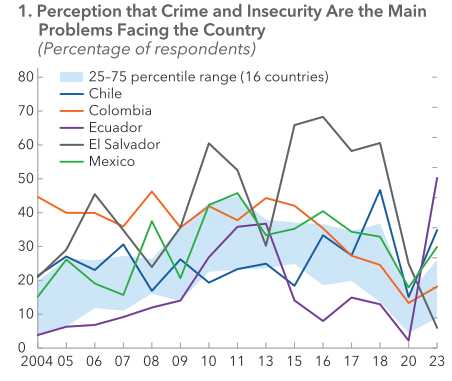
\includegraphics[width=0.7\textwidth]{images/inseguridad2024.png} % Adjust the width and file path
    \caption{Percepción de que la inseguridad es una prioridad \protect\cite{Bisca2024}}
    \label{fig:percepcion}
\end{figure}

La Figura \ref{fig:percepcion} muestra las prioridades con 
respecto al tiempo de la población en diferentes países 
latinoamericanos. La percepción de la prioridad de la violencia 
venía en decadencia desde el 2004, mientras que en los 
últimos 5 años, esta percepción ha mostrado una tendencia 
exponencialmente incremental. En este sentido, en la actualidad, 
la violencia representa la prioridad más importante que 
cualquier gobierno debería abordar. Por esta razón, en este 
proyecto se aborda la solución de este problema a través de la
detección de violencia interpersonal directa, a través del uso 
de inteligencia artificial. 

\section{Soluciones Clásicas}\label{solucionesClásicas}







\section{Detección de violencia a través de IA}\label{detecciónIA}
\thispagestyle{fancy}
En la presente sección, se detallan las arquitecturas y 
procedimientos para comprender mejor tanto el problema
de investigación como la solución propuesta. Entre estos
conocimientos previos, se explican en detalle algunas 
arquitecturas de CNN ampliamente usadas en la clasificación 
de imágenes utilizando ML, así como el procedimiento de 
\textit{Transfer Learning} (TL) y el preprocesamiento de 
entradas. \\

\subsection{\textit{Convolutional Neural Networks} (CNN)}

Las CNN son modelos basados en una arquitectura diseñada
específicamente para el análisis de imágenes, en particular
la clasificación. Estas realizan la tarea de extracción de
características a través de convoluciones. Esto evita la 
pérdida de información y mejora tanto la eficiencia como 
la precisión.\\

Las convoluciones se basan en un procedimiento que extrae
características mediante la aplicación de una pequeña matriz
de transformación cuadrada sobre la imagen original, la cual
retorna una imagen modificada. Estas matrices de transformación
se denominan kernels. La Figura \ref{convolucion} ilustra una
iteración de convolución.\\

\begin{figure}[h!] 
    \includegraphics[width=0.7\textwidth]{images/convolución.png} 
    \centering 
    \caption{Proceso simplificado de una convolución\protect\cite{convoluciones}.} 
    \label{convolucion} 
\end{figure}

Por otro lado, existen otras capas importantes llamadas
\textit{poolings}, como se muestra en la Figura \ref{pooling}.
Estas capas aplican una lógica a un cuadrante de la matriz
resultante de las convoluciones. Esta lógica varía dependiendo
de las necesidades del usuario. La Figura \ref{pooling} muestra una comparación
entre \textit{Max Pooling} y \textit{Average Pooling}, que obtienen
respectivamente los valores máximos y promedios de los cuadrantes
seleccionados para generar un nuevo resultado con menor dimensionalidad.

\begin{figure}[h!] 
    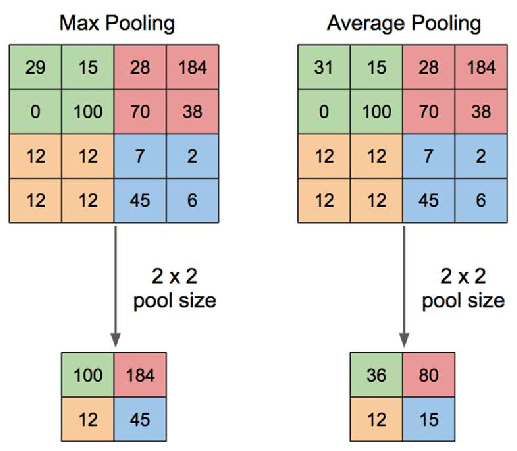
\includegraphics[width=0.6\textwidth]{images/pooling.png} 
    \centering 
    \caption{Proceso simplificado de un pooling \protect\cite{pooling}.} 
    \label{pooling} 
\end{figure}

Las CNN están compuestas por combinaciones repetidas de capas
convolucionales y de \textit{pooling}, finalizando en un conjunto 
de capas densas de neuronas llamadas \textit{Multi Layer 
Perceptron}(MLP), que realiza el procesamiento final de las 
características extraídas. La Figura \ref{CNN} muestra la 
estructura de una CNN. Como se mencionó anteriormente, 
la extracción de características se realiza dentro de la 
propia red neuronal, evitando la pérdida de información que 
se observa en los MLP y dejando únicamente la tarea de 
clasificación a estos últimos.

\begin{figure}[h!] 
    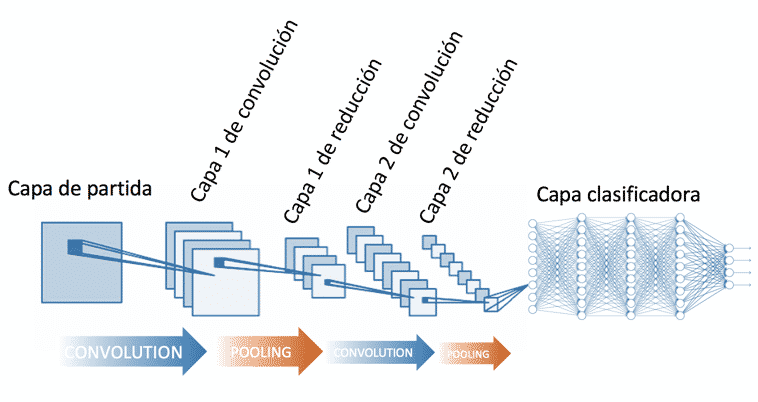
\includegraphics[width=1\textwidth]{images/CNN.png} 
    \centering 
    \caption{Arquitectura de una CNN convencional \protect\cite{CNN-Arquitectura}.} 
    \label{CNN} 
\end{figure}

A continuación, se explican cada una de las arquitecturas que 
son utilizadas en el presente trabajo. 

\section{VGG-19} 

Esta CNN tiene una profundidad de 19 capas y fue
creada por Karen Simonyan y Andrew Zisserman \cite{Simonyan2015}
en la Universidad de Oxford en 2014, y publicada posteriormente
en 2015. Su versión detallada se ilustra en la Figura \ref{VGG19}.
Este modelo fue utilizado para clasificar imágenes en el
\textit{dataset} ImageNet, logrando clasificar hasta 1000 objetos
diferentes. Espera una imagen de entrada de 224x224 píxeles para
su procesamiento. Debido a su profundidad, este modelo es bastante
pesado, llegando a consumir hasta 550 MB de memoria con alrededor
de 143 millones de parámetros. Cabe destacar que el 70\% de estos
parámetros se encuentran entre la última capa convolucional y la
primera capa de clasificación. Con todas estas características,
logró un 90\% de precisión en ImageNet.


\begin{figure}[h!] 
    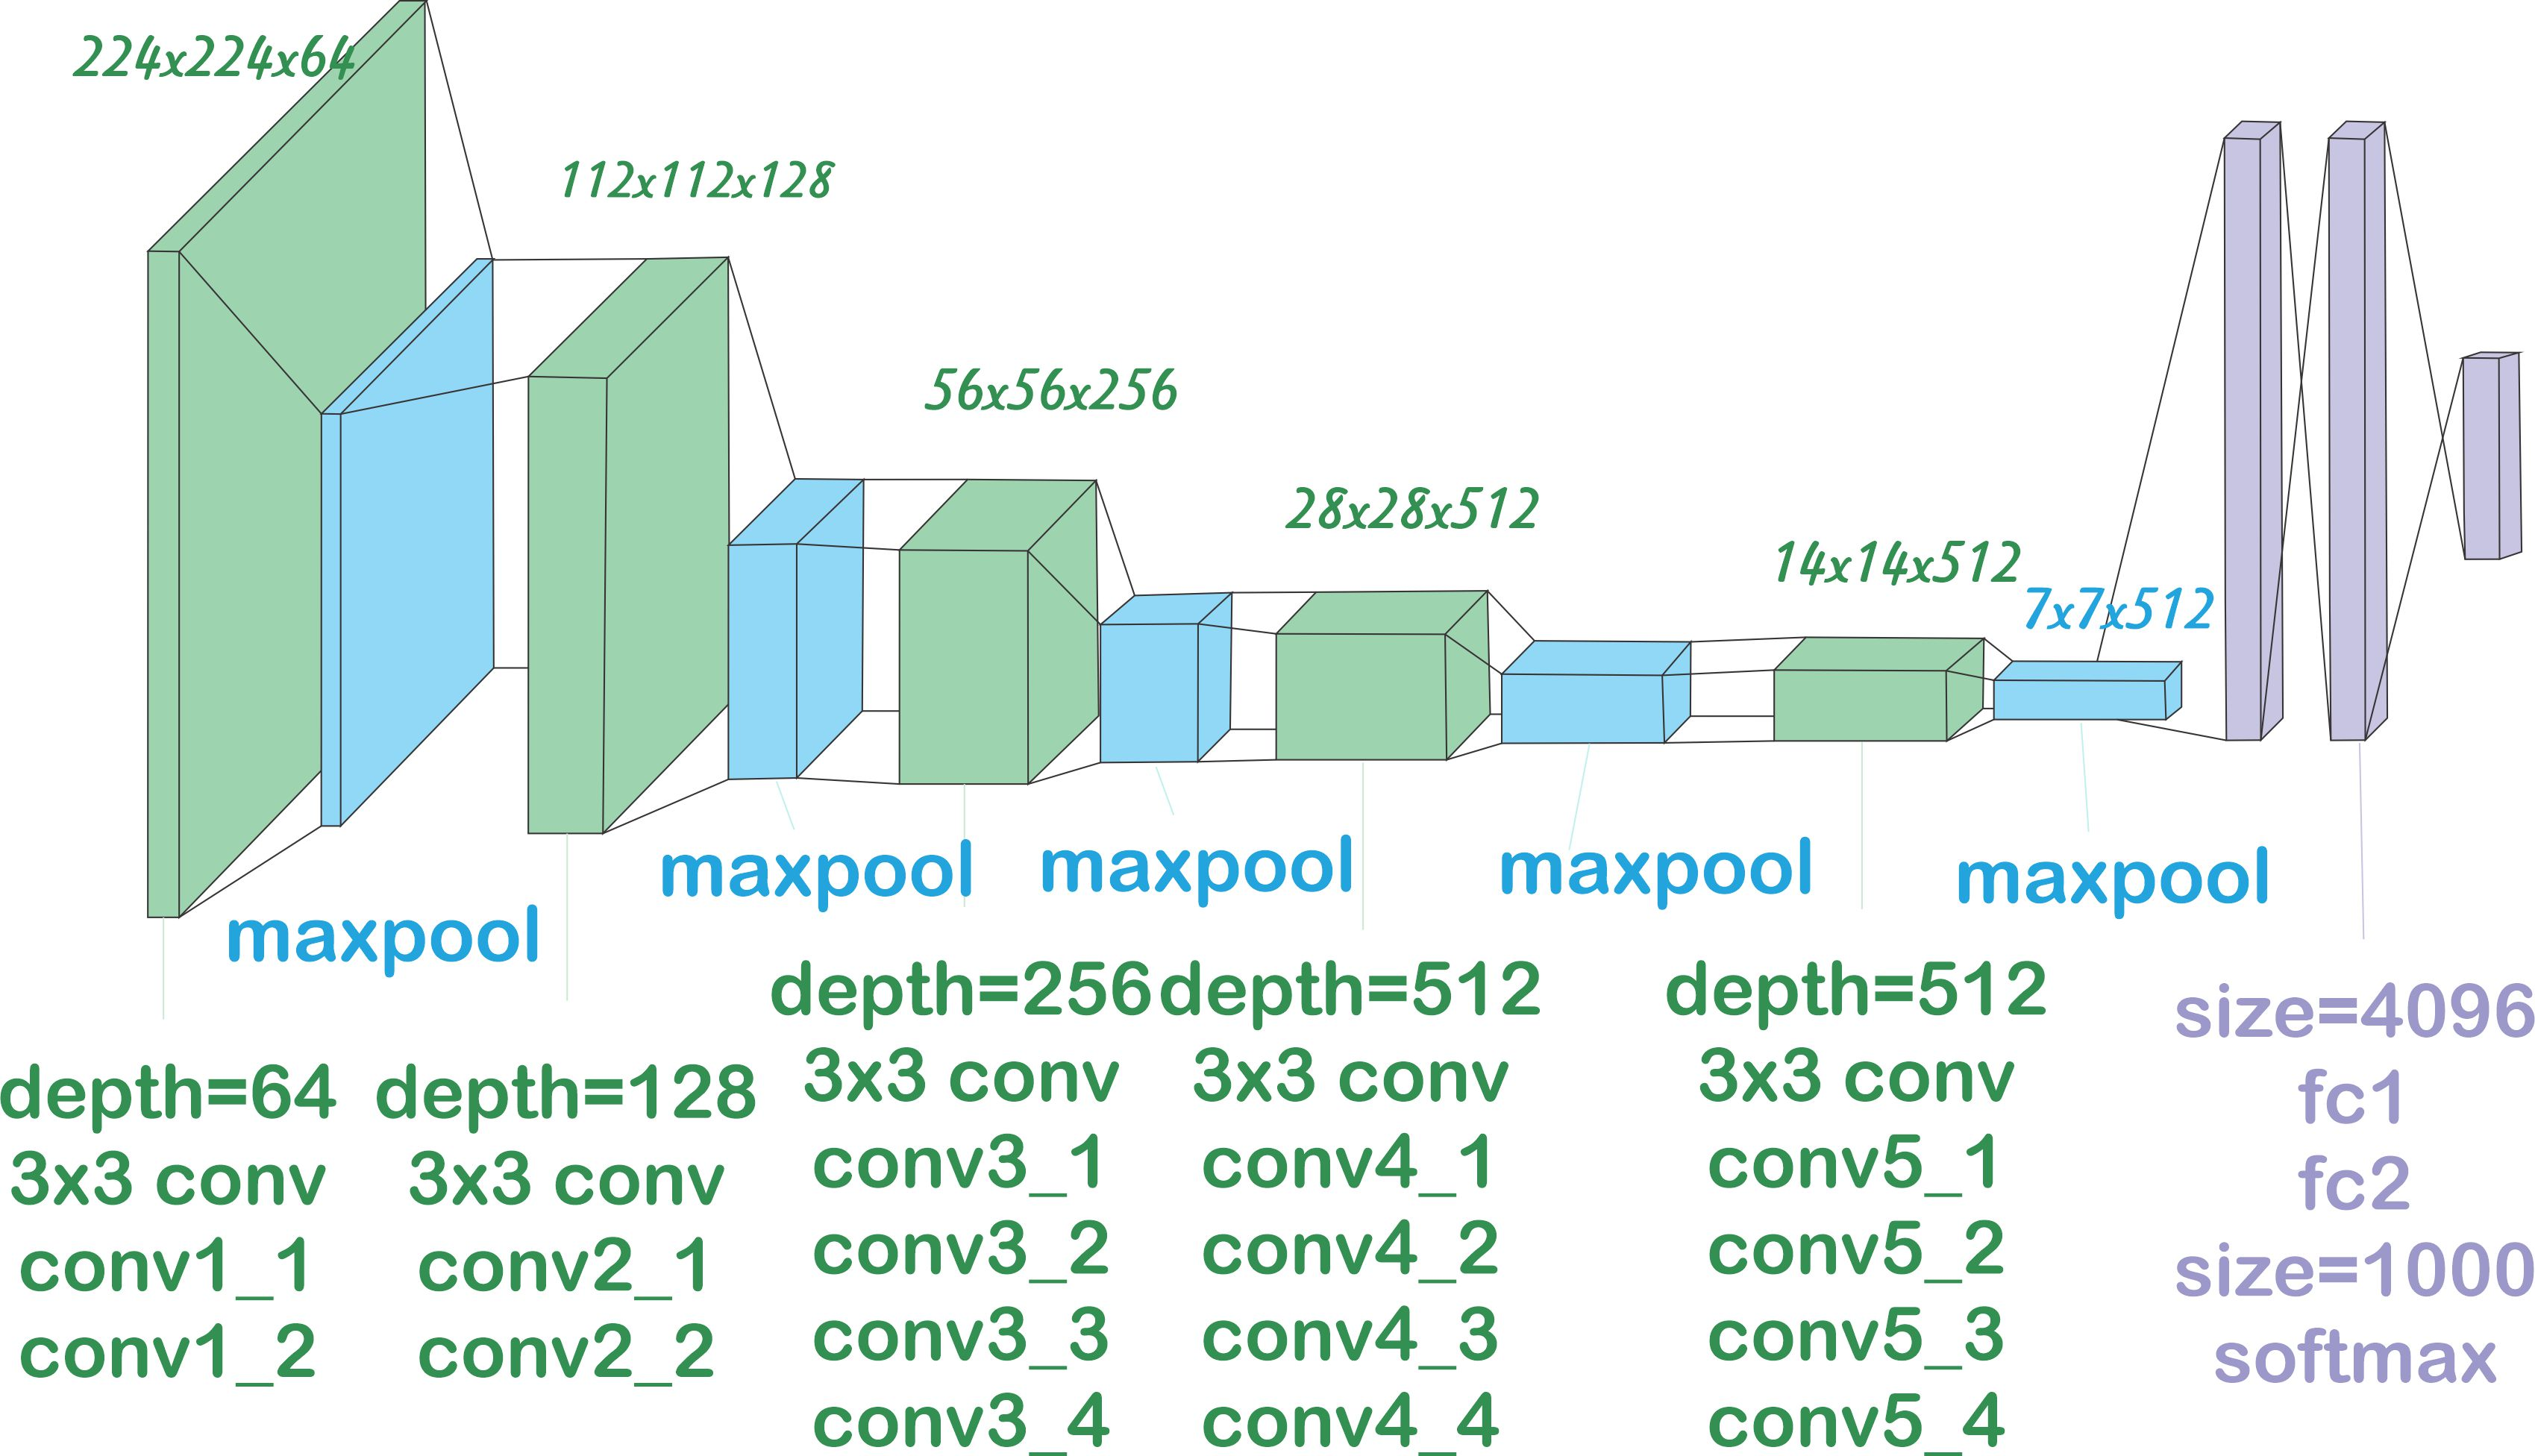
\includegraphics[width=1\textwidth]{images/VGG19.jpeg} 
    \centering 
    \caption{Version simplificada de una VGG19 \protect\cite{modelos}.} 
    \label{VGG19} 
\end{figure}


\section{InceptionV3} \label{sec:inceptionV3}
Aunque VGG19 logró una alta precisión, consumía demasiados
recursos. Por esta razón, Google desarrolló InceptionV3, una
red que prometía resultados similares pero a un menor costo.
Presentado en ``\textit{Going deeper with convolutions}''
\cite{Szegedy2014}, este modelo alcanza un 93.7\% de precisión
en el mismo \textit{dataset}.\

Aunque esta red tiene 50 capas de profundidad (más que VGG19),
tiene menos parámetros entrenables (23.8 millones). Su diseño
propuso que realizar convoluciones unidimensionales en serie
(como se muestra en la Figura \ref{InceptionLayer}) es
equivalente a una convolución bidimensional, evitando el uso
de filtros matriciales. Esto redujo la complejidad de los
modelos CNN convencionales, haciéndolo más liviano en memoria
y mejorando su capacidad de aprendizaje. En total, este modelo
pesa 92 MB—aproximadamente seis veces menos que el anterior.
Requiere imágenes de entrada de 299x299 píxeles, y su
arquitectura se muestra en la Figura \ref{Inceptionv3}.


\begin{figure}[h!] 
    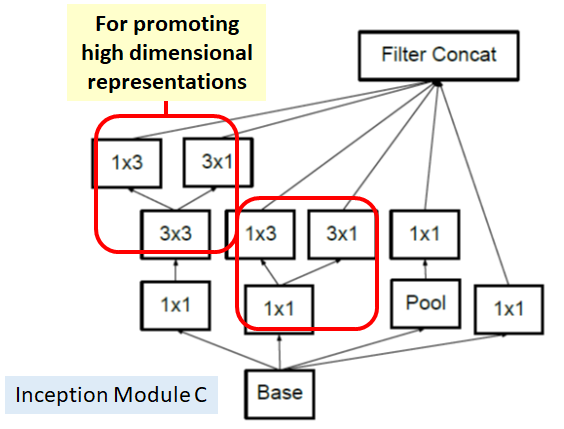
\includegraphics[width=0.8\textwidth]{images/InceptionLayer.png} 
    \centering 
    \caption{Reducción de dimensionalidad de InceptionV3 \protect\cite{modelos}.} 
    \label{InceptionLayer} 
\end{figure}

\begin{figure}[h!] 
    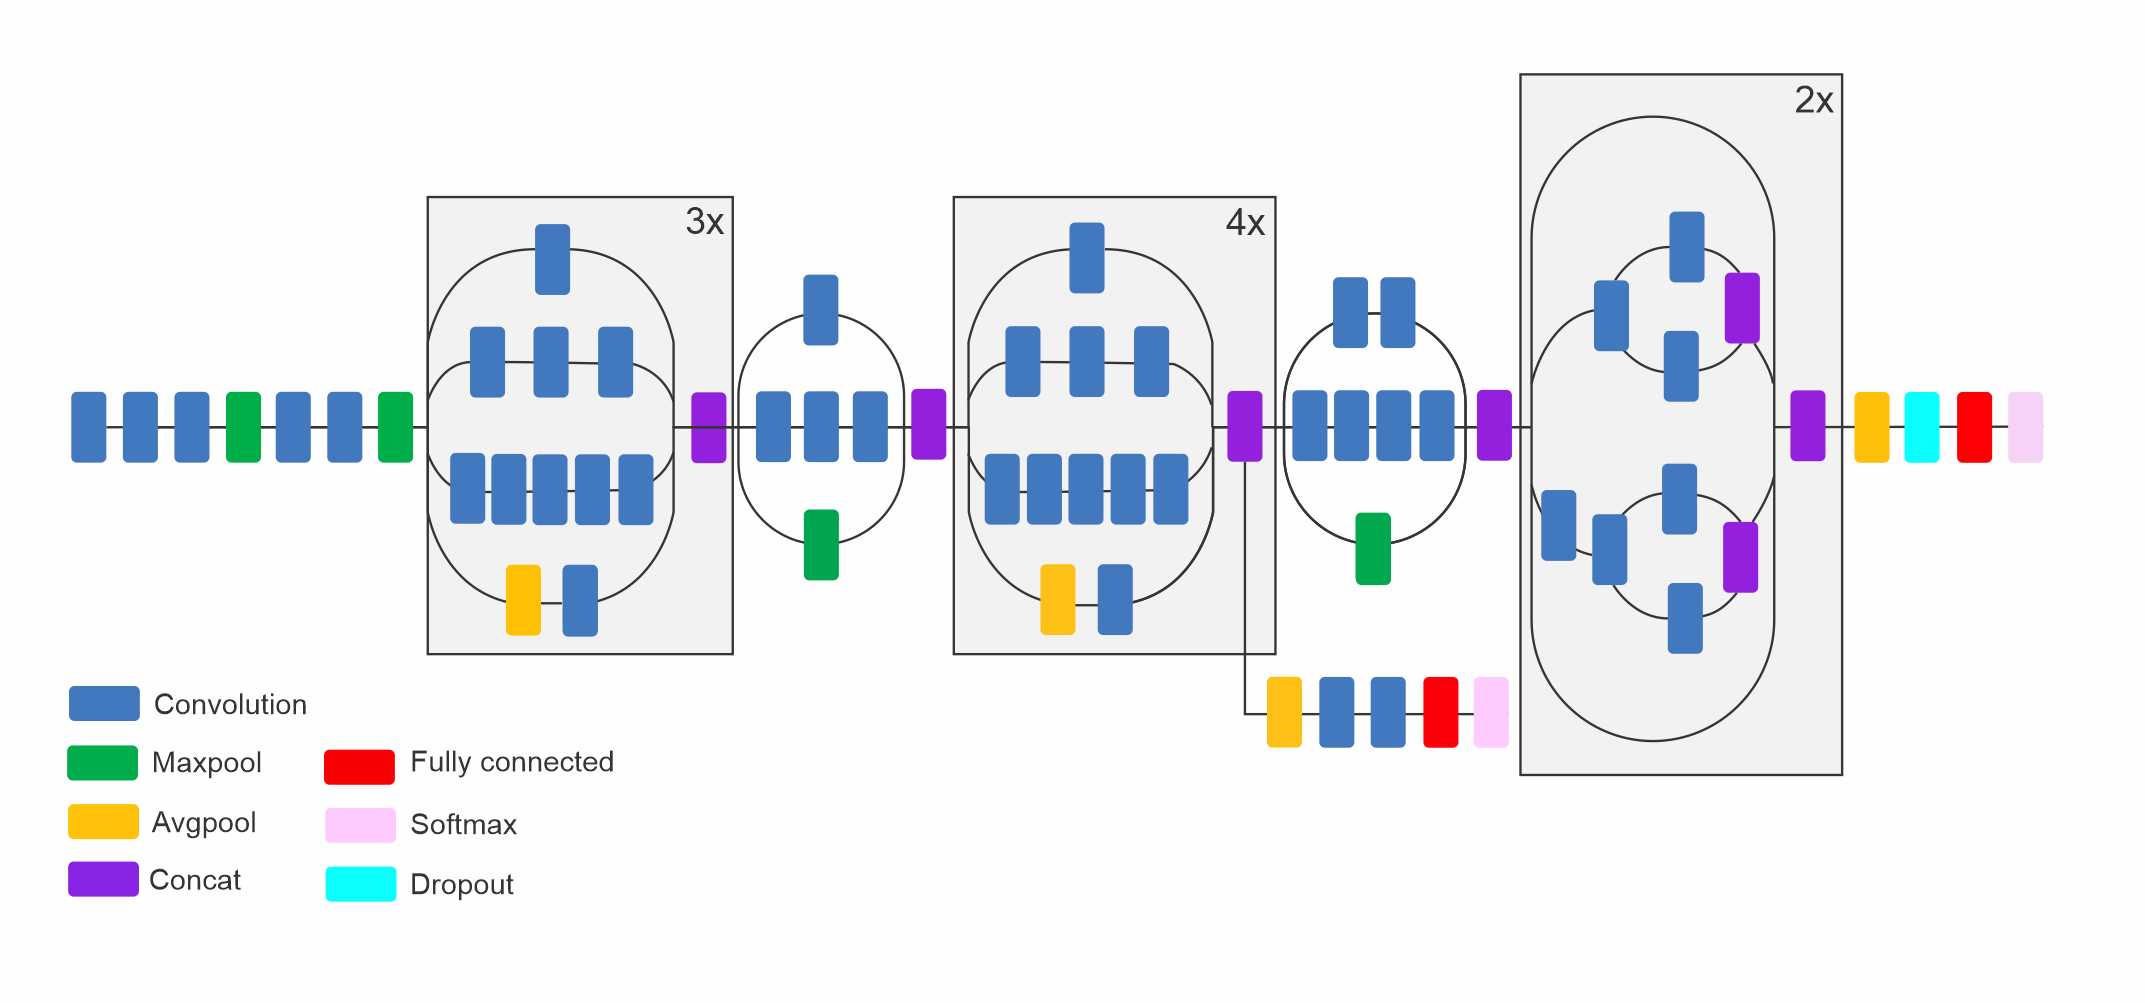
\includegraphics[width=1\textwidth]{images/InceptionV3.png} 
    \centering 
    \caption{Versión simplificada de InceptionV3 \protect\cite{modelos}.} 
    \label{Inceptionv3} 
\end{figure}

\section{ResNet50} 
Creado por Microsoft en 2015, este modelo también cuenta con 50 capas de
profundidad. Emplea una técnica llamada “residual learning”
\cite{He2015}, que consiste en guardar una copia de la salida actual y
sumarla al resultado obtenido de un conjunto de convoluciones (típicamente
cada tres). La Figura \ref{ResNet} ilustra esta modificación y la arquitectura
general del modelo. Este modelo también fue probado en el mismo
\textit{dataset}, obteniendo una precisión del 92.1\%, y el aprendizaje
residual evitó un aumento en la dimensionalidad del modelo.
Contiene aproximadamente 25.6 millones de parámetros y ocupa 98 MB de memoria.

\begin{figure}[h!] 
    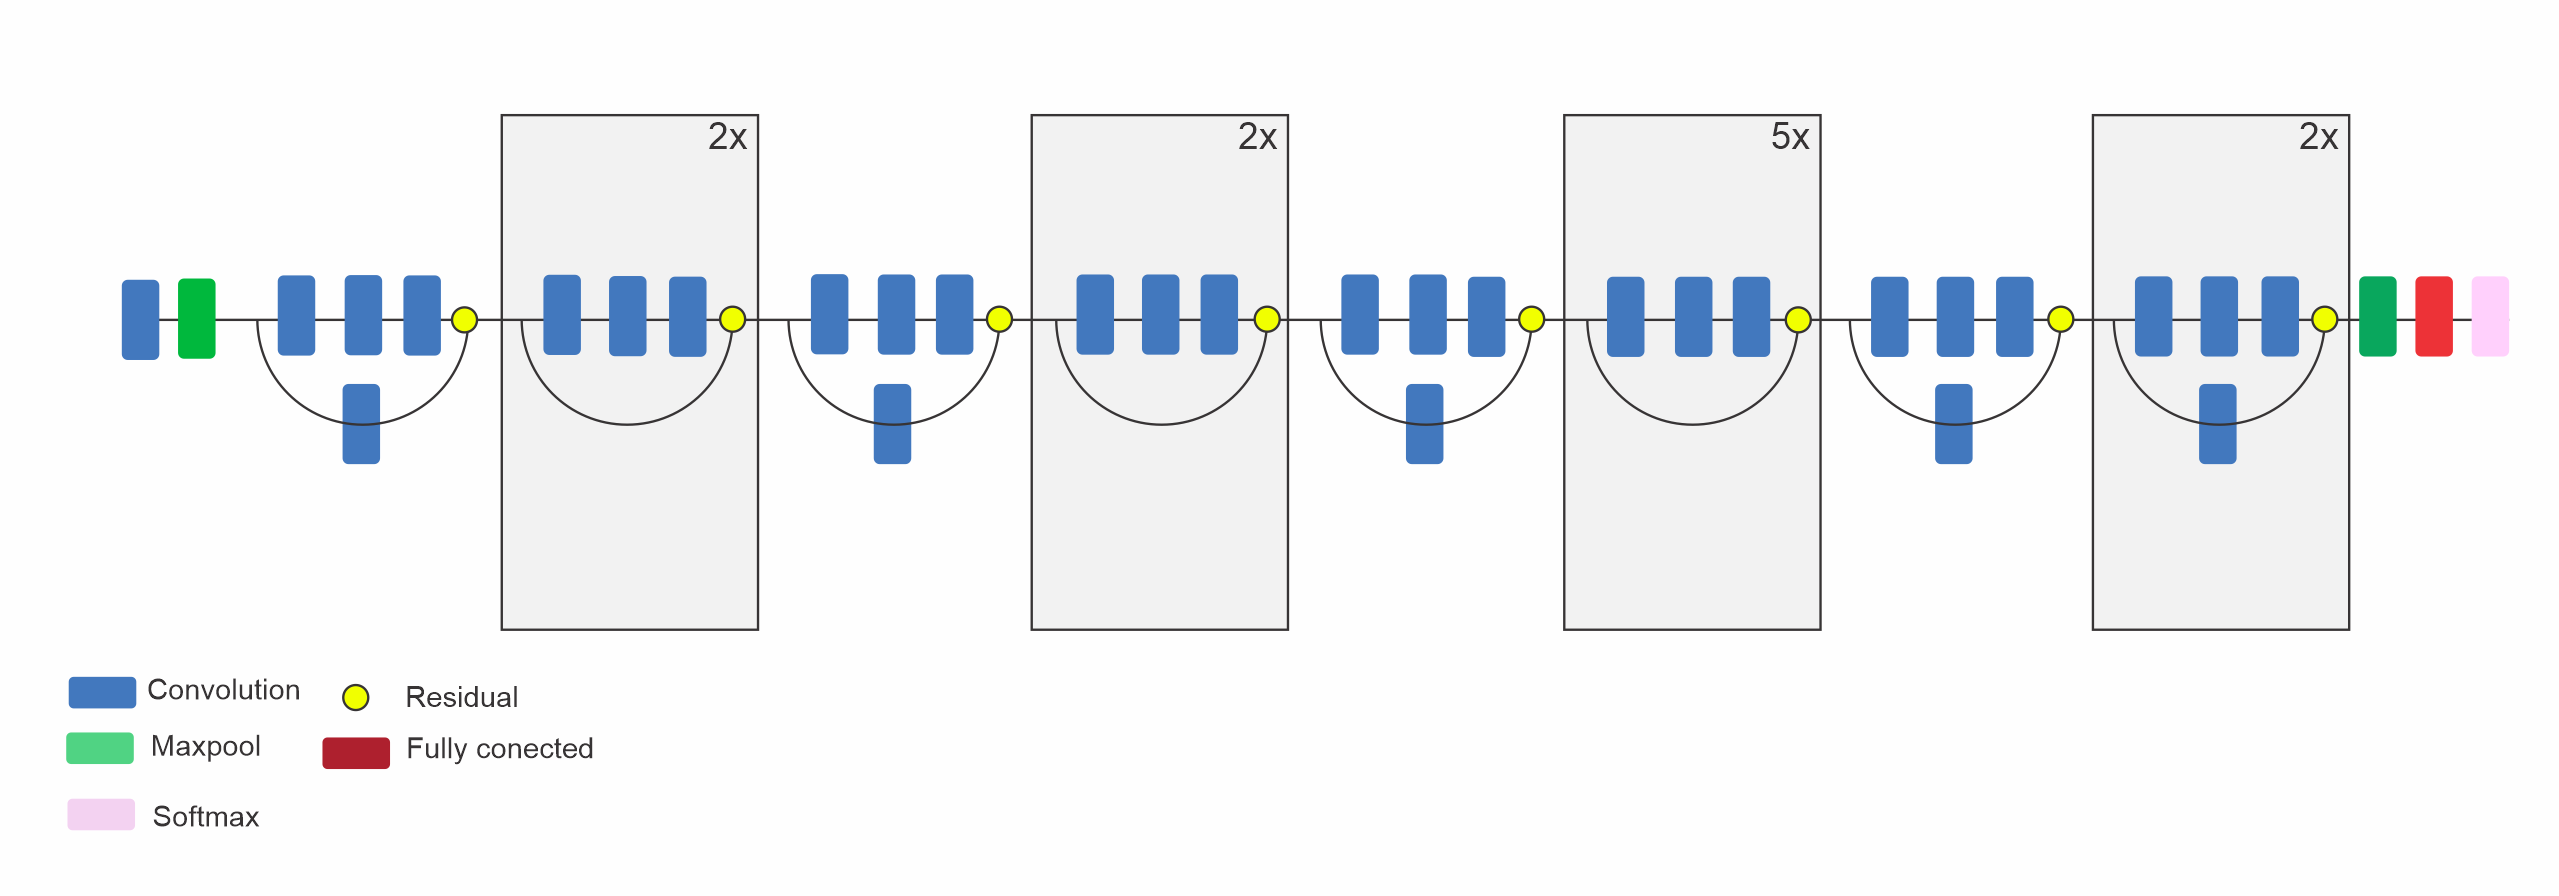
\includegraphics[width=1\textwidth]{images/ResNet.png} 
    \centering 
    \caption{Versión simplificada de ResNet50 \protect\cite{modelos}.} 
    \label{ResNet} 
\end{figure}

\section{EfficientNet} 
``\textit{EfficientNet: Rethinking Model Scaling for 
Convolutional Neural Networks}''\cite{Tan2020} en 2020, 
consiste en 8 implementaciones diferentes (B0 a B7).
La versión más ligera (B0) contiene aproximadamente 5.5 
millones de parámetros y logró un 93\% de precisión en el 
mismo \textit{dataset}. Otras versiones continúan aumentando 
el número de parámetros y la precisión resultante. Comparado 
con los modelos anteriores, EfficientNetB4 con 19.5 millones 
de parámetros alcanza un 96.4\% de precisión, superándolos.
Este modelo optimiza su aprendizaje mediante un algoritmo de 
aproximación que genera parámetros para crear cada uno de 
los ocho modelos. Este algoritmo considera tres factores:

\begin{itemize} 
    \item Profundidad de las capas 
    \item Ancho de las capas (capas múltiples) 
    \item Resolución de la imagen 
\end{itemize} 

La Figura \ref{EfficientNetB0} muestra la estructura de 
EfficientNetB0.

\begin{figure}[h!] 
    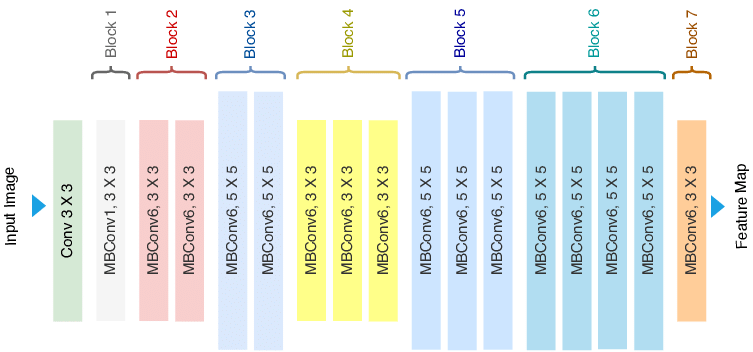
\includegraphics[width=1\textwidth]{images/EfficientNetB0.png} 
    \centering 
    \caption{Versión simplificada de EfficientNetB0 \protect\cite{EfficientNetB0}.} 
    \label{EfficientNetB0} 
\end{figure}

\section{YOLO} 
YOLO (\textit{you only look once}) es una arquitectura que 
permite la ``predicción simultánea de múltiples \textit{bounding boxes} 
y probabilidades de clase para ellas'' \cite{Redmon2015}. 
Este modelo está basado en una CNN convencional, que, a diferencia 
de implementaciones anteriores (R-CNN y FR-CNN), realiza la 
predicción de la caja de enlace internamente, reduciendo la latencia 
y habilitando su uso en tiempo real.\\

Este cálculo se basa en generar cuadrículas o particiones de la 
imagen, dentro de las cuales se inicializa un número predeterminado 
de \textit{bounding boxes} predefinidas (ambos son hiperparámetros de la 
arquitectura). Esto es replicable usando cualquier arquitectura 
CNN como base (por ejemplo, uno de los modelos mencionados previamente), 
solo ajustando la salida y los hiperparámetros en consecuencia. 
Las versiones más recientes logran una mejor detección, módulos de 
atención y otras variaciones que la hacen cada vez más robusta. 
La Figura \ref{YOLO} muestra un ejemplo de la arquitectura del modelo 
YOLOv5.

\begin{figure}[h!] 
    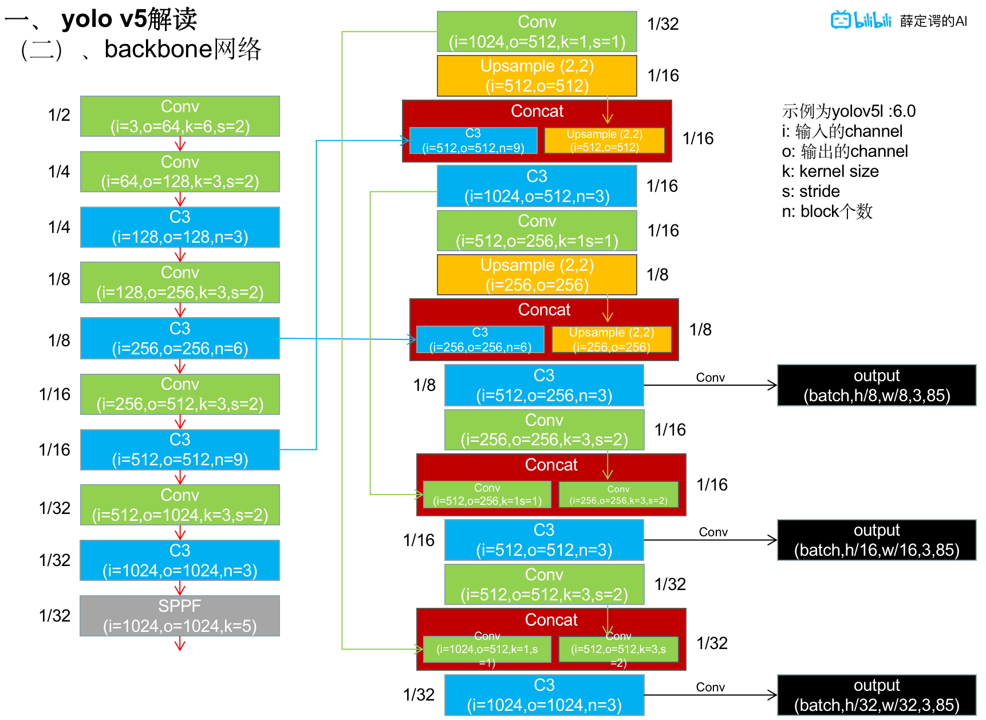
\includegraphics[width=1\textwidth]{images/yolov5.png} 
    \centering 
    \caption{Representación de la arquitectura de YOLOv5\protect\cite{yolov5}.} 
    \label{YOLO} 
\end{figure}

\section{\textit{Long Short-Term Memory} (LSTM)}

Las redes \textit{Long Short-Term Memory} (LSTM) fueron 
desarrolladas como una extensión de las redes neuronales 
recurrentes (RNN) con el propósito de superar la dificultad 
de aprender dependencias a largo plazo en secuencias
\cite{hochreiter1997lstm}. Las 
RNN tradicionales tienden a sufrir del problema del 
desvanecimiento o explosión del gradiente durante el 
proceso de entrenamiento, lo que limita su capacidad 
para capturar relaciones temporales distantes. Las LSTM 
abordan esta limitación mediante la incorporación de una 
memoria interna controlada por compuertas, lo que permite 
conservar información relevante a lo largo del tiempo.

La arquitectura de las LSTM se basa en una celda de memoria 
capaz de mantener su estado a lo largo de múltiples pasos 
temporales. Esta celda está regulada por tres compuertas 
fundamentales: la compuerta de entrada, que controla qué 
nueva información se almacena en la celda; la compuerta 
de olvido, que decide qué información debe eliminarse 
del estado anterior; y la compuerta de salida, que 
determina qué parte del contenido de la celda se utiliza 
como salida. Estas compuertas permiten que la red aprenda a 
retener o descartar información de manera adaptativa, mejorando 
significativamente el aprendizaje de secuencias largas.

Gracias a esta estructura, las LSTM han demostrado un 
rendimiento notable en una amplia gama de tareas secuenciales 
donde el contexto temporal es esencial. Aplicaciones como 
el modelado del lenguaje natural, la traducción automática, 
el reconocimiento de voz y el análisis de series temporales 
se han beneficiado enormemente de su capacidad para capturar 
dependencias a largo plazo. En consecuencia, las LSTM se han 
convertido en una arquitectura fundamental dentro del campo 
del aprendizaje profundo secuencial.La arquitectura de este modelo se puede ver en la imagen 
\ref{lstm}:

\begin{figure}[h!] 
    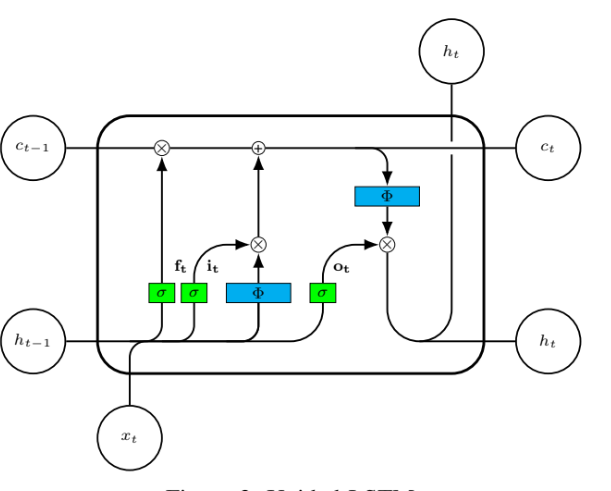
\includegraphics[width=1\textwidth]{images/lstm.png} 
    \centering 
    \caption{Representación de la arquitectura de LSTM\protect\cite{datascientest2024lstm}.} 
    \label{lstm} 
\end{figure}


\subsection{\textit{Transfer Learning}}
Según Muhamad Yani \cite{Yani2019}, 
\textit{Transfer Learning (TL)} se define como ``el proceso de 
transferir el conocimiento de un entrenamiento previo para ser 
utilizado en un nuevo modelo con el fin de reducir el tiempo de 
aprendizaje''. Este proceso puede ser observado en la Figura 
\ref{transfer-learning}.\\

\begin{figure}[h!]
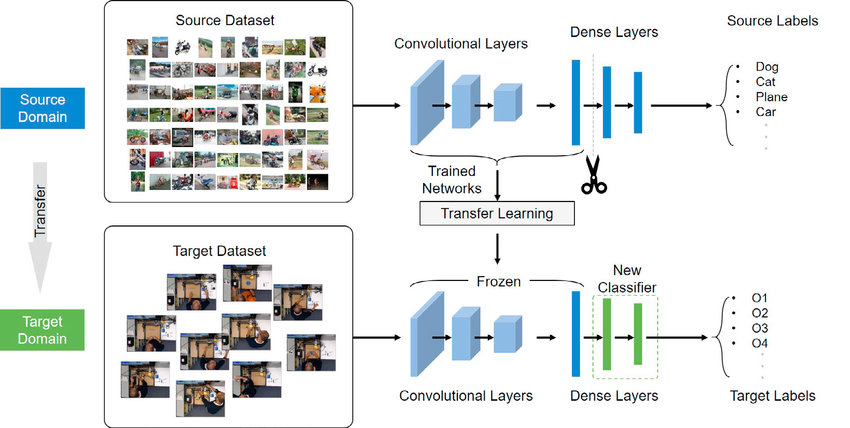
\includegraphics[width=1\textwidth]{images/transfer-learning.png}
\centering
\caption{Comparativa entre un entrenamiento normal y por TL\protect\cite{transfer-learning}.}
\label{transfer-learning}
\end{figure}
TL difiere del proceso de entrenamiento convencional de una 
red en que no es necesario entrenarla con un gran conjunto de 
datos. A diferencia del proceso tradicional, las capas iniciales 
del modelo (en nuestro caso, las capas convolucionales) están 
congeladas. Estas capas contienen todo el conocimiento pre-aprendido 
del conjunto de datos con el cual el modelo fue originalmente entrenado. 
Una vez obtenidas esas capas, se agregan nuevas capas densas (similares 
a las de un MLP) que sirven como clasificadores para nuestro propósito 
específico. Gracias a esto, solo las capas finales necesitan ser entrenadas, 
lo que requiere menos datos y generalmente resulta en predicciones precisas. 
Este tipo de entrenamiento se llama ``\textit{fine-tuning}'', lo que permite 
que la red ajuste el aprendizaje previo para predecir en función de un conjunto 
de datos diferente al que fue entrenada originalmente, ahorrando tiempo y 
mejorando la precisión.

\subsection{Preprocesamiento de Entradas}
Ahora que entendemos cómo funcionan estos modelos en general, 
necesitamos observar las características requeridas de las 
entradas para que el modelo aprenda de manera efectiva.

\subsubsection{Tamaño de la Entrada}
Considerando solo las diferentes CNN, cada modelo espera una 
matriz de entrada (imagen) de un tamaño específico. En las 
implementaciones actuales, se usan comúnmente tensores para 
referirse a un \textit{batch} (conjunto) de imágenes. La 
representación es la siguiente:

$$(batch, channels, m, n), donde:$$
\begin{itemize}
    \item batch: Número de imágenes que se ingresan a la vez.
    \item channels: Número de canales de la imagen (para imágenes a color, hay 3 canales que representan RGB, mientras que las imágenes en escala de grises tienen solo 1 canal).
    \item m \& n: Dimensiones de la imagen. Estos valores dependen de la arquitectura del modelo, ya que cada capa realizará operaciones que reducen la dimensionalidad de la imagen. Esto varía según la implementación debido a las diversas configuraciones posibles para cada matriz convolucional y operación de pooling.
\end{itemize}

\subsubsection{\textit{One Hot Encoder}}
Este es un tipo de representación que consiste en crear una 
matriz identidad de tamaño $n \times n$, donde $n$ es 
el número de \textit{etiquetas}. La codificación de cada 
etiqueta puede tomarse como una de las filas de la matriz. 
Así, podemos representar la codificación de un objeto de 
la clase j entre n clases como:

$$OneHotEncoder(i,j,n)= [a_1,a_2, .. a_n], donde: $$
\begin{equation*}
a_{i,j}=
\begin{cases}
1 & \text{si j = i}\\
0 &  \text{otherwise}
\end{cases}
\end{equation*}
Este tipo de codificación tiene la ventaja de evitar 
relaciones entre etiquetas, y permite una clasificación 
sencilla al comparar resultados. En el lado negativo, 
puede llevar a una alta dimensionalidad cuando hay muchas 
\textit{etiquetas}.

\subsection{\textit{Overfitting}}
El proceso de aprendizaje de los modelos se basa en la retroalimentación 
obtenida a través de la retropropagación mencionada anteriormente. 
Una vez que se actualizan los pesos de cada neurona utilizando el 
gradiente resultante, se puede decir que el modelo ha aprendido 
a clasificar esa imagen específica. Sin embargo, este gradiente 
puede desvanecerse debido a la profundidad de la arquitectura, 
las funciones de activación u otras razones. Este gradiente 
desvanecido impide que el modelo siga aprendiendo del 
conjunto de datos, lo que lo hace inutilizable para aplicaciones 
del mundo real. Algunas estrategias utilizadas para abordar 
esto son:

\begin{itemize}
    \item {\textit{Data Augmentation}: Expansión del conjunto 
    de datos original utilizando rotaciones, escalados, recortes, 
    volteos, etc. Esto hace que el modelo sea más resistente 
    a los cambios en la posición o orientación del objeto en la imagen.}
    \item {\textit{Batch Normalization}: Reescalado de los datos 
    de entrada a diferentes rangos relativos a una escala común, 
    generando una distribución de datos más manejable.}
    \item {\textit{Dropout}: Desactivación aleatoria de un 
    porcentaje de neuronas artificiales en una capa. Esto 
    impide que cada neurona dependa de las desactivadas, 
    mejorando generalmente el rendimiento.}
\end{itemize}

Este capítulo presentó los conocimientos previos que 
ayudarán a los lectores a comprender mejor la metodología 
que se introducirá más adelante particularmente las arquitecturas de 
los modelos que se revisarán, utilizarán y compararán para 
lograr los mejores resultados posibles en la detección y clasificación 
de imágenes de peces dentro de la fauna marina peruana.



\subsection{\textit{Pipelines} actuales para la clasificacion de violencia}

La literatura actual muestra un creciente interés en la 
detección automática de violencia en videos mediante la 
combinación de redes convolucionales (CNN) y redes de 
memoria a largo plazo (LSTM). Las CNN se utilizan para extraer 
características espaciales relevantes de los fotogramas, 
permitiendo identificar patrones visuales y contextos que podrían 
indicar situaciones violentas. Posteriormente, estas 
características son procesadas por las LSTM, las cuales se 
encargan de capturar la dinámica temporal y las dependencias 
de largo plazo entre los fotogramas, mejorando la capacidad 
de detectar eventos violentos que se desarrollan a lo largo 
del tiempo.\\

En diversos estudios se ha demostrado que la integración 
de ambas arquitecturas permite explotar de forma sinérgica 
las ventajas de cada una: las CNN fortalecen la comprensión 
del contenido visual a nivel de detalle y textura, mientras 
que las LSTM aportan una perspectiva temporal que es crucial 
para identificar patrones de comportamiento complejos y 
secuenciales propios de la violencia. Este tipo de 
\textit{pipeline} ha sido evaluado en diferentes escenarios, 
incluyendo videos de vigilancia y grabaciones deportivas, 
logrando así mejores tasas de detección en comparación con 
métodos que utilizan únicamente análisis espacial o temporal 
de manera aislada.\\

Un claro ejemplo de lo mencionado anteriormente, 
es el artículo de Jeff Donahue, \textit{et al.}
\cite{Donahue2016}. Su investigación se centra en el 
desafío de trabajar con datos visuales que contienen 
información espacial y temporal. La idea central es 
integrar ambas arquitecturas en un único sistema 
end-to-end: las CNNs se encargan de extraer 
representaciones ricas de contenido visual, y las 
LSTMs modelan la dinámica secuencial, permitiendo 
aplicaciones en reconocimiento de actividades en video y 
generación de descripciones de imágenes. \\

Entre sus principales contribuciones, este trabajo 
logró sentar las bases las bases en la integración de 
arquitecturas visuales y secuenciales. Su enfoque ha 
influido en numerosos trabajos posteriores en áreas como 
la descripción automática de videos, el análisis de 
secuencias complejas y el desarrollo de modelos más 
integrados para tareas multimodales.\\

Utilizando esta lógica, el trabajo de Orozco, \textit{et al.}\cite{Orozco2021} el cual 
destaca la efectividad de estas estrategias al combinar 
etapas de preprocesamiento, extracción de características 
espaciales mediante CNN, y análisis secuencial temporal con 
LSTM. Asimismo, se discuten los desafíos asociados a la 
variabilidad de escenarios y la detección en tiempo real, 
aspectos que continúan motivando la investigación y 
optimización de estos sistemas. Como resultado final de su 
experimentación, los autores lograron un F1-score de 91\% 
lo cual indica que fue \textit{pipeline} robusto el 
problema que intentó resolver basado en la clasificación de 
acciones humanas basado en videos. Los pipelines híbridos 
basados en CNN y LSTM representan una tendencia robusta en 
el campo de la detección de violencia, contribuyendo 
significativamente a la mejora en la precisión y eficiencia 
de los sistemas de análisis de video.\\

Otro artículo que también utiliza esta misma lógica es el de
Swathikiran Sudhakaran and Oswald Lanz\cite{Sudhakaran2017}. Su objetivo consistió 
en el mismo del presente trabajo, la detección de violencia. 
Para ello, se utilizó el \textit{dataset} de Hockey Fights, 
el cuál contiene videos de eventos violentos en partidos de 
hockey. Este \textit{dataset} es bastante usado como \textit{benchmark} 
y consiste de un conjunto de imágenes etiquetadas de manera 
homogenea. La variación más significativa que realizaron fue el 
uso de celdas convLSTM en vez de LSTM regulares para poder 
obtener un \textit{accuracy} más elevado. Con su \textit{pipeline} 
lograron obtener una \textit{accuracy} de 97\%, generando un 
nuevo record para este \textit{benchmark} y marcando un nuevo 
estado del arte. \\


De la misma manera y utilizando el mismo \textit{dataset} de 
Hockey Fights, se encuentra el trabajo de Al-Maamoon R. Abdali 
y Rana F. Al-Tuma\cite{Abdali2019}. Ellos se basaron en el 
trabajo anteriormente mencionado para su implementación. 
Para ello, utilizaron la misma configuración del 
\textit{pipeline} pero incluyeron capas 
conv3d y 40 celdas para el aprendizaje de la LSTM sin ser 
convolucionales. Utilizando aquella configuración logrando 
obtener un \textit{accuracy} de 96.33\% 
pero al mismo tiempo obteniendo una mejora de 4 veces en la 
velocidad (representado en el número de fps), representando 
una mejora del estado del arte en su tiempo al mantener el 
mismo nivel de \textit{accuracy} pero mejorando el 
\textit{performance}.\\


El último artículo a revisar es el de Patel Mann 
\cite{Mann2021}. En su trabajo utilizó Resnet50, InceptionV3 
y VGG19 como extractores de características. En cambio, 
utilizaron solo una celda LSTM para la clasificación y como 
resultados obtuvieron 90\% de precisión para 
el dataset de Hockey fights, representando una disminución a 
comparación de los anteriores trabajos, aunque permitió optimizar 
el uso de memoria sin perder drásticamente el \textit{performance} 
de todo el \textit{pipeline}.\\

Como se puede ver, el \textit{pipeline} CNN-LSTM propuesto ha 
sido utilizado a lo largo de los últimos años para resolver 
problemas similares e iguales al nuestro. En ese sentido nos hace 
sentido tratar de extender la aplicación de este y optimizarlo 
para tratar de ver como es que diferentes configuraciones del 
mismo permiten mejorar ya sea el \textit{performance} o el 
\textit{accuracy} de la propuesta.



\chapter{Objetivos}
\section{Objetivos}
En este capítulo se presentarán los objetivos y contribuciones de 
esta tesis. Una comprensión clara de estos aspectos es 
esencial para contextualizar el alcance y la relevancia de 
esta investigación. Las siguientes secciones ofrecerán una 
discusión detallada de los objetivos clave perseguidos en 
este trabajo, así como de las contribuciones que se pretende 
aportar al campo.
\begin{itemize}
  \item { Objetivo principal: 
      \begin{itemize}
          \item optimizar el equilibrio entre la modificación 
          del extractor de características CNN y el ajuste del 
          número de celdas LSTM para construir el pipeline más 
          efectivo para la detección de violencia
      \end{itemize}
   }
   \item { Objetivos secundarios:
      \begin{itemize}
          \item Evaluar el impacto de diversas arquitecturas 
          CNN en la calidad de las características 
          espaciotemporales extraídas para la detección de 
          violencia.
          \item Investigar cómo la variación en el número 
          de celdas LSTM afecta la modelación temporal y el 
          rendimiento en la clasificación.
          \item Identificar el equilibrio óptimo entre la 
          complejidad de la extracción de características por 
          CNN y la capacidad de las LSTM para lograr el mejor 
          rendimiento con un costo computacional mínimo.
          \item Automatizar el proceso de etiquetado mediante la 
          creación de una aplicación en tiempo real para el pipeline.
      \end{itemize}
      }
\end{itemize}

\section{Contribuciones}

La contribución principal de esta tesis es el desarrollo de 
un pipeline optimizado para la detección de violencia que 
equilibra la complejidad de la extracción de características 
basada en CNN y el número de celdas LSTM para lograr una 
mayor precisión y eficiencia. Al analizar sistemáticamente 
los compromisos entre estos dos componentes, este trabajo 
proporciona un enfoque estructurado para diseñar arquitecturas 
de deep learning destinadas al reconocimiento espaciotemporal 
de violencia, mejorando tanto el rendimiento en la detección 
como la viabilidad computacional. Esta contribución tiene 
como objetivo avanzar en el análisis de video impulsado por 
IA para aplicaciones de vigilancia en tiempo real.


\chapter{Desarrollo del trabajo}
En el presente capítulo se explica la experimentación 
realizada para la clasificación de los videos del 
\textit{dataset Hockey Fights}. La 
estructura que se detalla a continuación consiste de: 
explicación del \textit{pipeline}, la experimentación 
con las diferentes configuraciones de BI-LSTM y la 
comparativa de los resultados.

En la Sección \ref{software} se explican las especificaciones de 
\textit{software} y \textit{hardware} que se necesitaron para la 
realización del trabajo.\\

Mientras que en la Sección \ref{experimentacion} se detallan todos los experimentos 
realizados con cada una de las diferentes configuraciones y sus 
resultados.\\

Por último, en la Sección {comparativa} se realiza la comparativa de 
todos los resultados obtenidos considerando el promedio y las mejores 
ejecuciones del \textit{pipeline} para finalmente poder obtener una 
conclusión acerca de la influencia del número de capas Bi-LSTM con 
respecto a los resultados finales obtenidos. 

\section{Software y Hardware}\label{software}

A lo largo de toda la experimentación, se utiliza
un computador de escritorio. Los detalles de la misma se encuentran en 
la Tabla \ref{caracteristicas}.

\begin{table}[h!]
\centering
\caption{Características del computador utilizado para el trabajo.}

\begin{tabular}{|r|r|}
\hline
\textbf{Componente} & \textbf{Descripción} \\ \hline
Procesador & AMD Ryzen 7 3700X 8-Core 3.6 GHz. \\ \hline
Memoria RAM & Crucial Ballistix 16GB DDR4 - 3600MHZ \\ \hline
Tarjeta Gráfica & Nvidia RTX 2060 6GB \\ \hline
\end{tabular}
\label{caracteristicas}
\end{table}

Por otra parte, se utilizó Python, junto con Keras, Sklearn y Tensorflow 
para el desarrollo del \textit{pipeline} en general y el pre y post 
procesamiento de los datos. Para el procesamiento de las imágenes (con Yolo) 
se utilizó OpenCV compilado con cudnn para la habilitación del uso de tarjeta gráfica. 

\section{Experimentación} \label{experimentacion}

La presente Sección se subdivide en dos partes: la Sección \ref{procesamiento} 
revisa la creación de la CNN encargada de extraer las características de cada uno 
de los frames, mientras que la Sección \ref{clasificacion} presenta la 
experimentación de las diferentes configuraciones de la Bi-LSTM con múltiples 
capas.\\

En la Sección \ref{procesamiento} se detallan los pasos del 
procesamiento, los resultados provenientes del mismo y una tabla 
comparativa con métricas específicas por modelo de CNN a utilizar. 

Mientras que en la Sección \ref{clasificacion} se detallan los 
resultados obtenidos de utilizar diferentes configuraciones de capas 
Bi-LSTM para clasificar los vectores característicos obtenidos de los 
\textit{frames}. 


\subsection{Preprocesamiento y obtención de características}\label{procesamiento}

Como primer paso, se procede a realizar el pre-procesamiento 
de las imágenes y la obtención de sus características tal 
como fue mencionado anteriormente. Para ello, se utilizan los modelos 
con sus pesos preentrenados con el \textit{dataset ImageNet}. Además, se 
congelan todas sus capas convolucionales y eliminan todas las demás. Por último 
se agrega una capa \textit{GlobalAveragePooling2D}. Una vez terminado, 
se recolectan las métricas acerca de la cantidad de parámetros y el 
tiempo de cálculo por batch de cada uno de los modelos, los cuales 
se puden observar en la Tabla \ref{tabla:preprocesamiento}:

\begin{table}[h!]
\centering
\caption{Tabla comparativa de los parámetros y tiempo de inferencia por modelo.}
\begin{tabular}{|l|l|l|}
\hline
\multicolumn{1}{|c|}{\textbf{Modelo}} & \multicolumn{1}{c|}{\textbf{Parámetros}} & \multicolumn{1}{c|}{\textbf{\begin{tabular}[c]{@{}c@{}}Timpo de inferencia\\ (por batch de 10)\\ en ms/batch\end{tabular}}} \\ \hline
\textbf{Efficientnetb0}               & 4,049,571                                & 46 ms                                                                                                                       \\ \hline
\textbf{Resnet50}                     & 23,587,712                               & 51 ms                                                                                                                       \\ \hline
\textbf{Efficientnetv2-s}             & 20,331,360                               & 75 ms                                                                                                                       \\ \hline
\textbf{MobilenetV3large}             & 2,996,352                                & 45 ms                                                                                                                       \\ \hline
\end{tabular}
\label{tabla:preprocesamiento}
\end{table}

Se puede apreciar que el tamaño final de los modelos fue 
menor que el esperado por la Tabla \ref{evaluacion}. 
Esto se debe a que no se están utilizando las capas densas 
de los modelos y se estan reemplazando con una capa 
GlobalAveragePooling2D, la cual obtiene el resultado del 
kernel final de las capas convolucionales y las reduce a un 
solo resultado promediado. 

\subsection{Clasificación de los videos a través de la Bi-LSTM}\label{clasificacion}

Después de obtener las características de cada uno de las 
imágenes y los diez frames generados por cada uno de ellas, 
se entrenan diferentes modelos BI-LSTM como fue mencionado 
anteriormente, teniendo desde 1 a 10 celdas para cada uno de 
las CNN utilizados tal como se menciona en la Sección 
\ref{pipeline}. A continuación se explican los resultados para cada 
una de los diferentes experimentos realizados.\\

\textbf{\underline{Resultados obtenidos con EfficientNetB0}}\\

La Tabla \ref{table:b0Metrics} muestra una comparativa 
entre los resultados obtenidos para el \textit{pipeline} manteniendo 
los vectores de características obtenidas a través de EfficientNetB0 
de los frames del \textit{dataset Hockey Fights}.\\

\begin{table}[h!]
\centering
\footnotesize
\caption{Métricas obtenidas por configuración de celdas para EfficientNetB0.}
\begin{tabular}{|l|l|l|l|l|l|l|}
\hline
\textbf{\begin{tabular}[c]{@{}l@{}}Celdas \\ Bi-LSTM\end{tabular}} & \textbf{\begin{tabular}[c]{@{}l@{}}Perdida \\ entrenamiento\end{tabular}} & \textbf{\begin{tabular}[c]{@{}l@{}}Accuracy \\ entrenamiento\end{tabular}} & \textbf{\begin{tabular}[c]{@{}l@{}}Perdida \\ validacion\end{tabular}} & \textbf{\begin{tabular}[c]{@{}l@{}}Accuracy \\ validacion\end{tabular}} & \textbf{\begin{tabular}[c]{@{}l@{}}Perdida \\ prueba\end{tabular}} & \textbf{\begin{tabular}[c]{@{}l@{}}Accuracy \\ prueba\end{tabular}} \\ \hline
\textbf{1}                                                         & 0.07                                                                      & 0.98                                                                       & 0.22                                                                   & 0.94                                                                    & 0.12                                                               & 0.97                                                                \\ \hline
\textbf{2}                                                         & 0.05                                                                      & 0.99                                                                       & 0.1                                                                    & 0.98                                                                    & 0.08                                                               & 0.98                                                                \\ \hline
\textbf{3}                                                         & 0.04                                                                      & 0.99                                                                       & 0.16                                                                   & 0.96                                                                    & 0.08                                                               & 0.98                                                                \\ \hline
\textbf{4}                                                         & 0.02                                                                      & 0.99                                                                       & 0.14                                                                   & 0.95                                                                    & 0.08                                                               & 0.97                                                                \\ \hline
\textbf{5}                                                         & 0.02                                                                      & 0.99                                                                       & 0.16                                                                   & 0.96                                                                    & 0.07                                                               & 0.98                                                                \\ \hline
\textbf{6}                                                         & \textbf{0.0}                                                              & \textbf{1.0}                                                               & \textbf{0.15}                                                          & \textbf{0.98}                                                           & \textbf{0.03}                                                      & \textbf{0.99}                                                       \\ \hline
\textbf{7}                                                         & 0.05                                                                      & 0.99                                                                       & 0.19                                                                   & 0.96                                                                    & 0.13                                                               & 0.96                                                                \\ \hline
\textbf{8}                                                         & 0.03                                                                      & 0.99                                                                       & 0.14                                                                   & 0.98                                                                    & 0.06                                                               & 0.99                                                                \\ \hline
\textbf{9}                                                         & 0.02                                                                      & 0.99                                                                       & 0.14                                                                   & 0.98                                                                    & 0.09                                                               & 0.98                                                                \\ \hline
\end{tabular}
\label{table:b0Metrics}
\end{table}


En la Tabla \ref{table:b0Metrics} se puede observar 
que los mejores resultados a lo largo de todos los pasos del 
\textit{pipeline} fue la configuración de 6 celdas, generando 99\% de 
\textit{accuracy} en prueba. Además, se pudo observar que los 
resultados de las demás configuraciones fueron similares a lo largo de 
todas las confguraciones, pero si se revisa los valores entre ellas, 
es claro que todos ellos empeoran mientras más se alejan de esa 
configuración, salvo en la configuración con 6 celdas que es un caso 
anómalo.\\

A continuación se presentan las gráficas de pérdida y \textit{accuracy} 
de esta configuración.

\begin{figure}[h!] 
    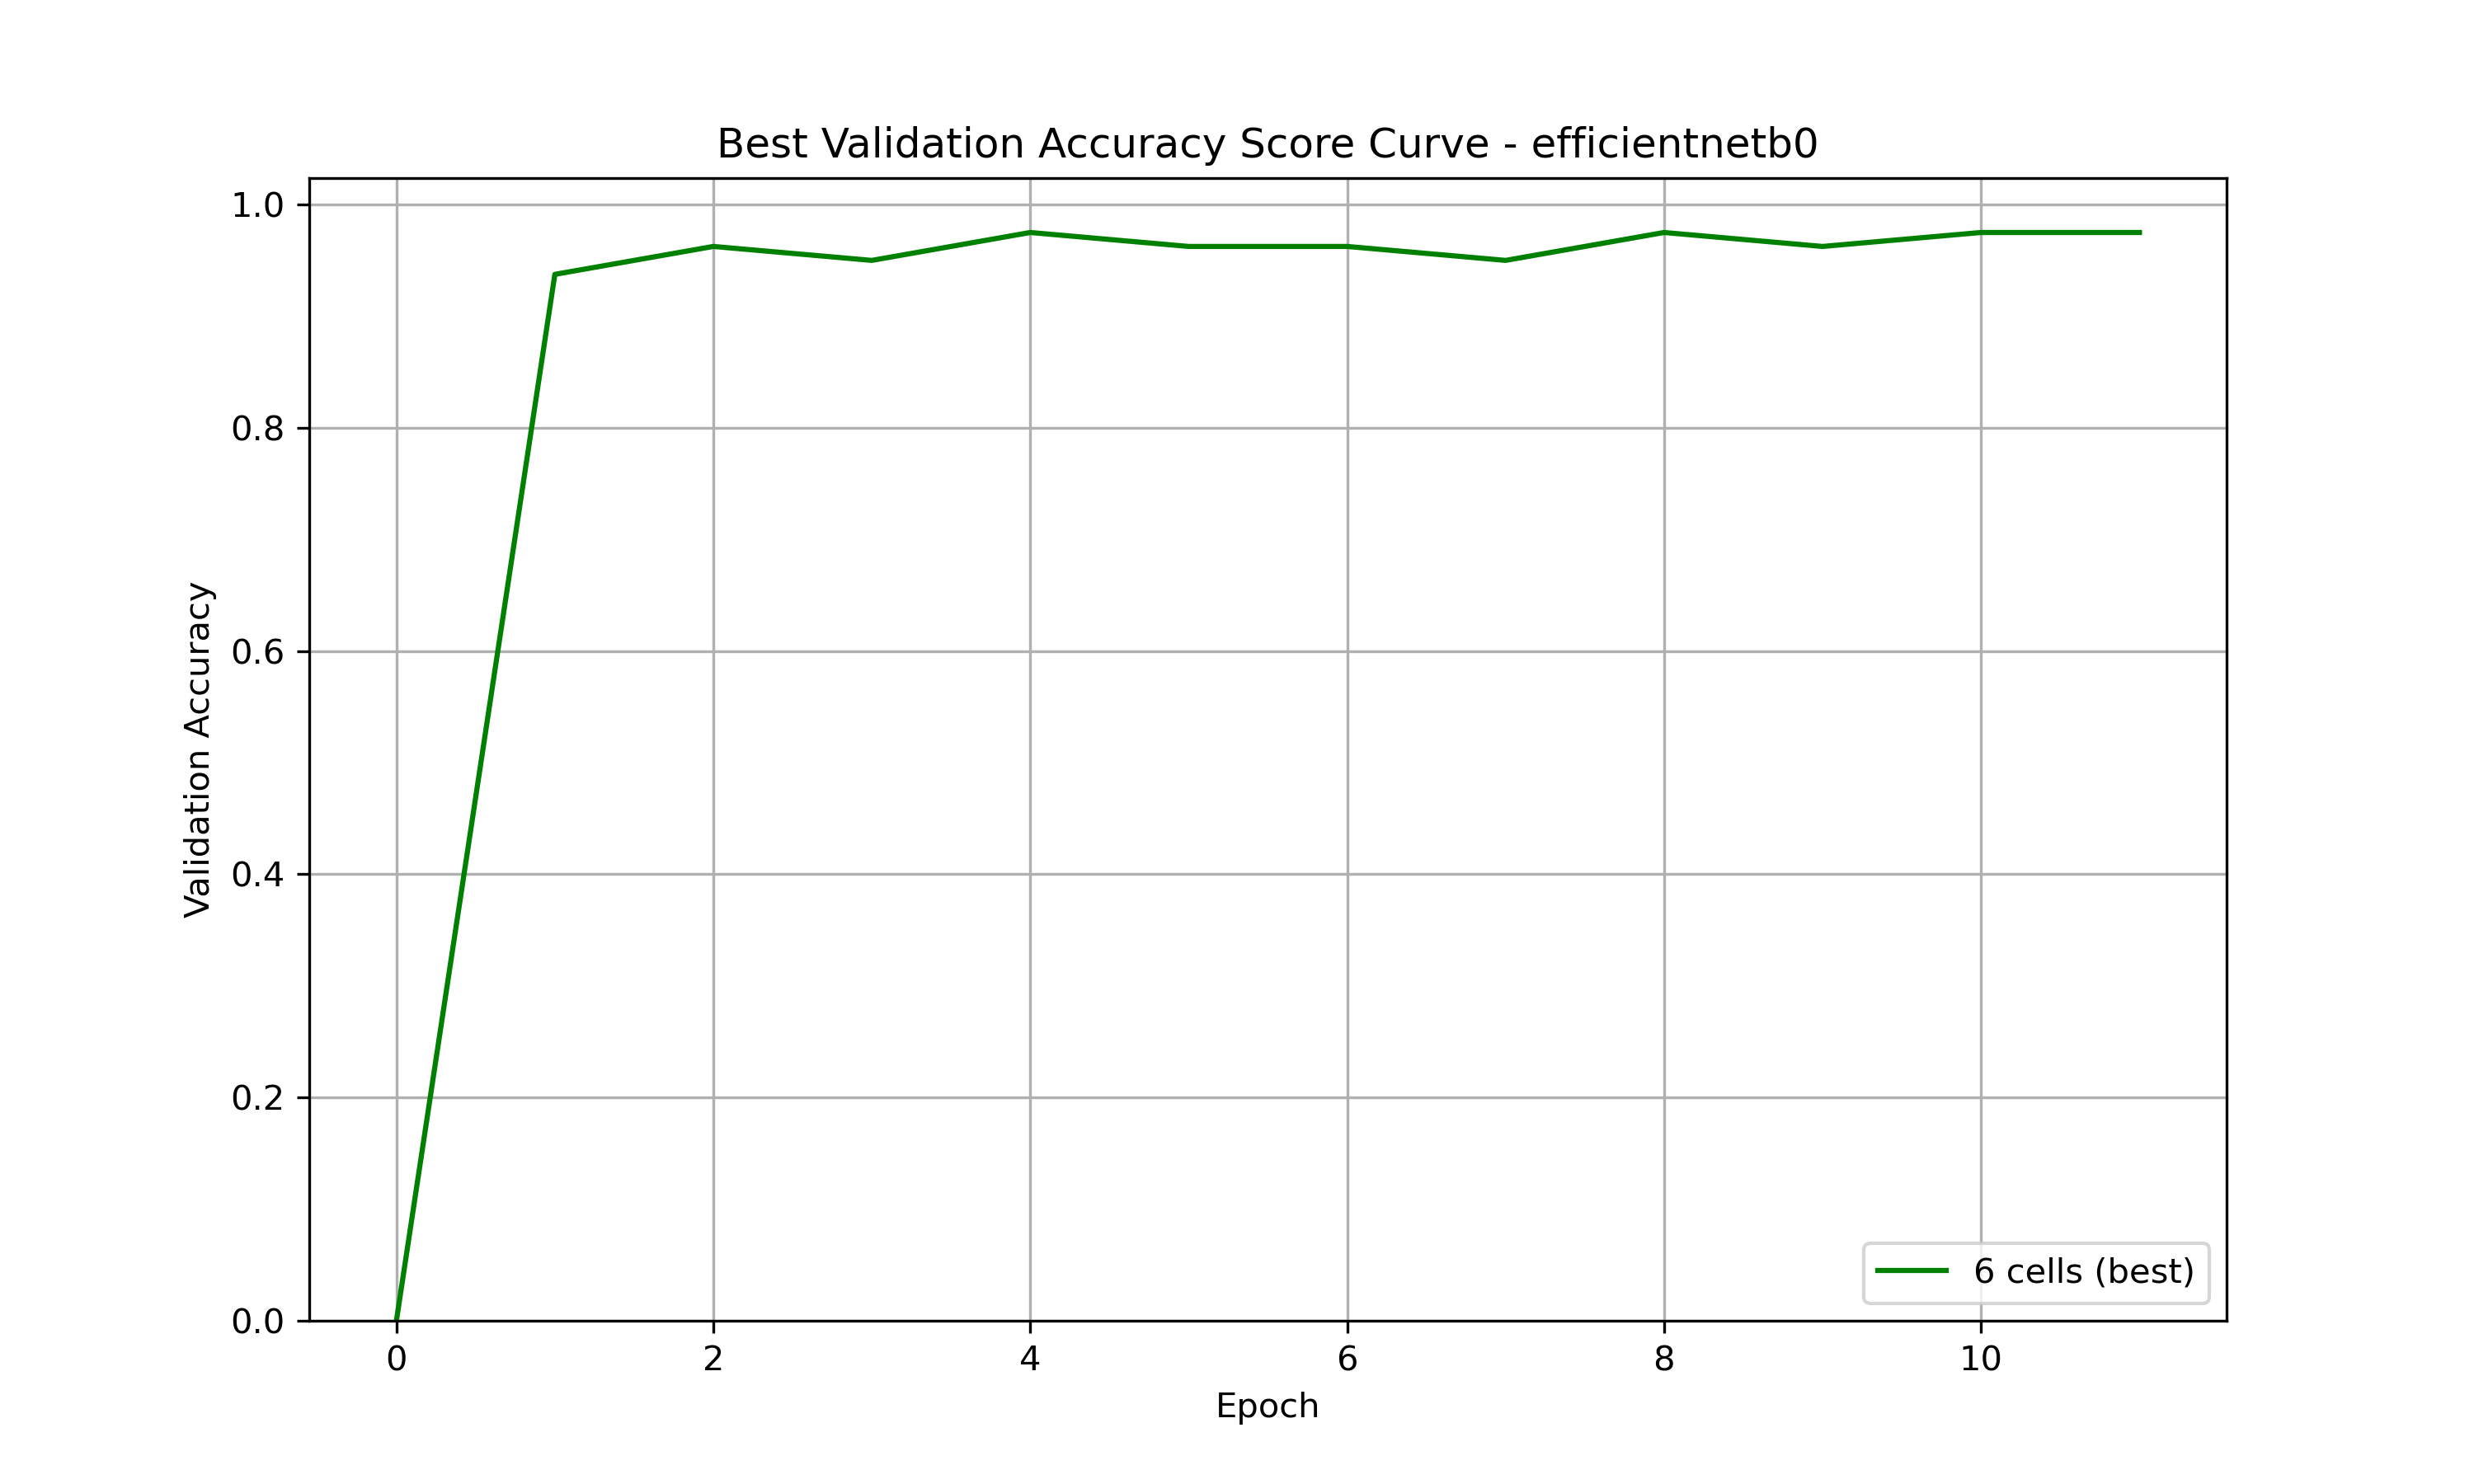
\includegraphics[width=0.8\textwidth]{../graphs/efficientnetb0_best_val_accuracy.png} 
    \centering 
    \caption{\textit{Accuracy} por época de EfficientNetB0 y 6 capas Bi-LSTM } 
    \label{EfficientNetB0Accuracy} 
\end{figure}

\begin{figure}[h!] 
    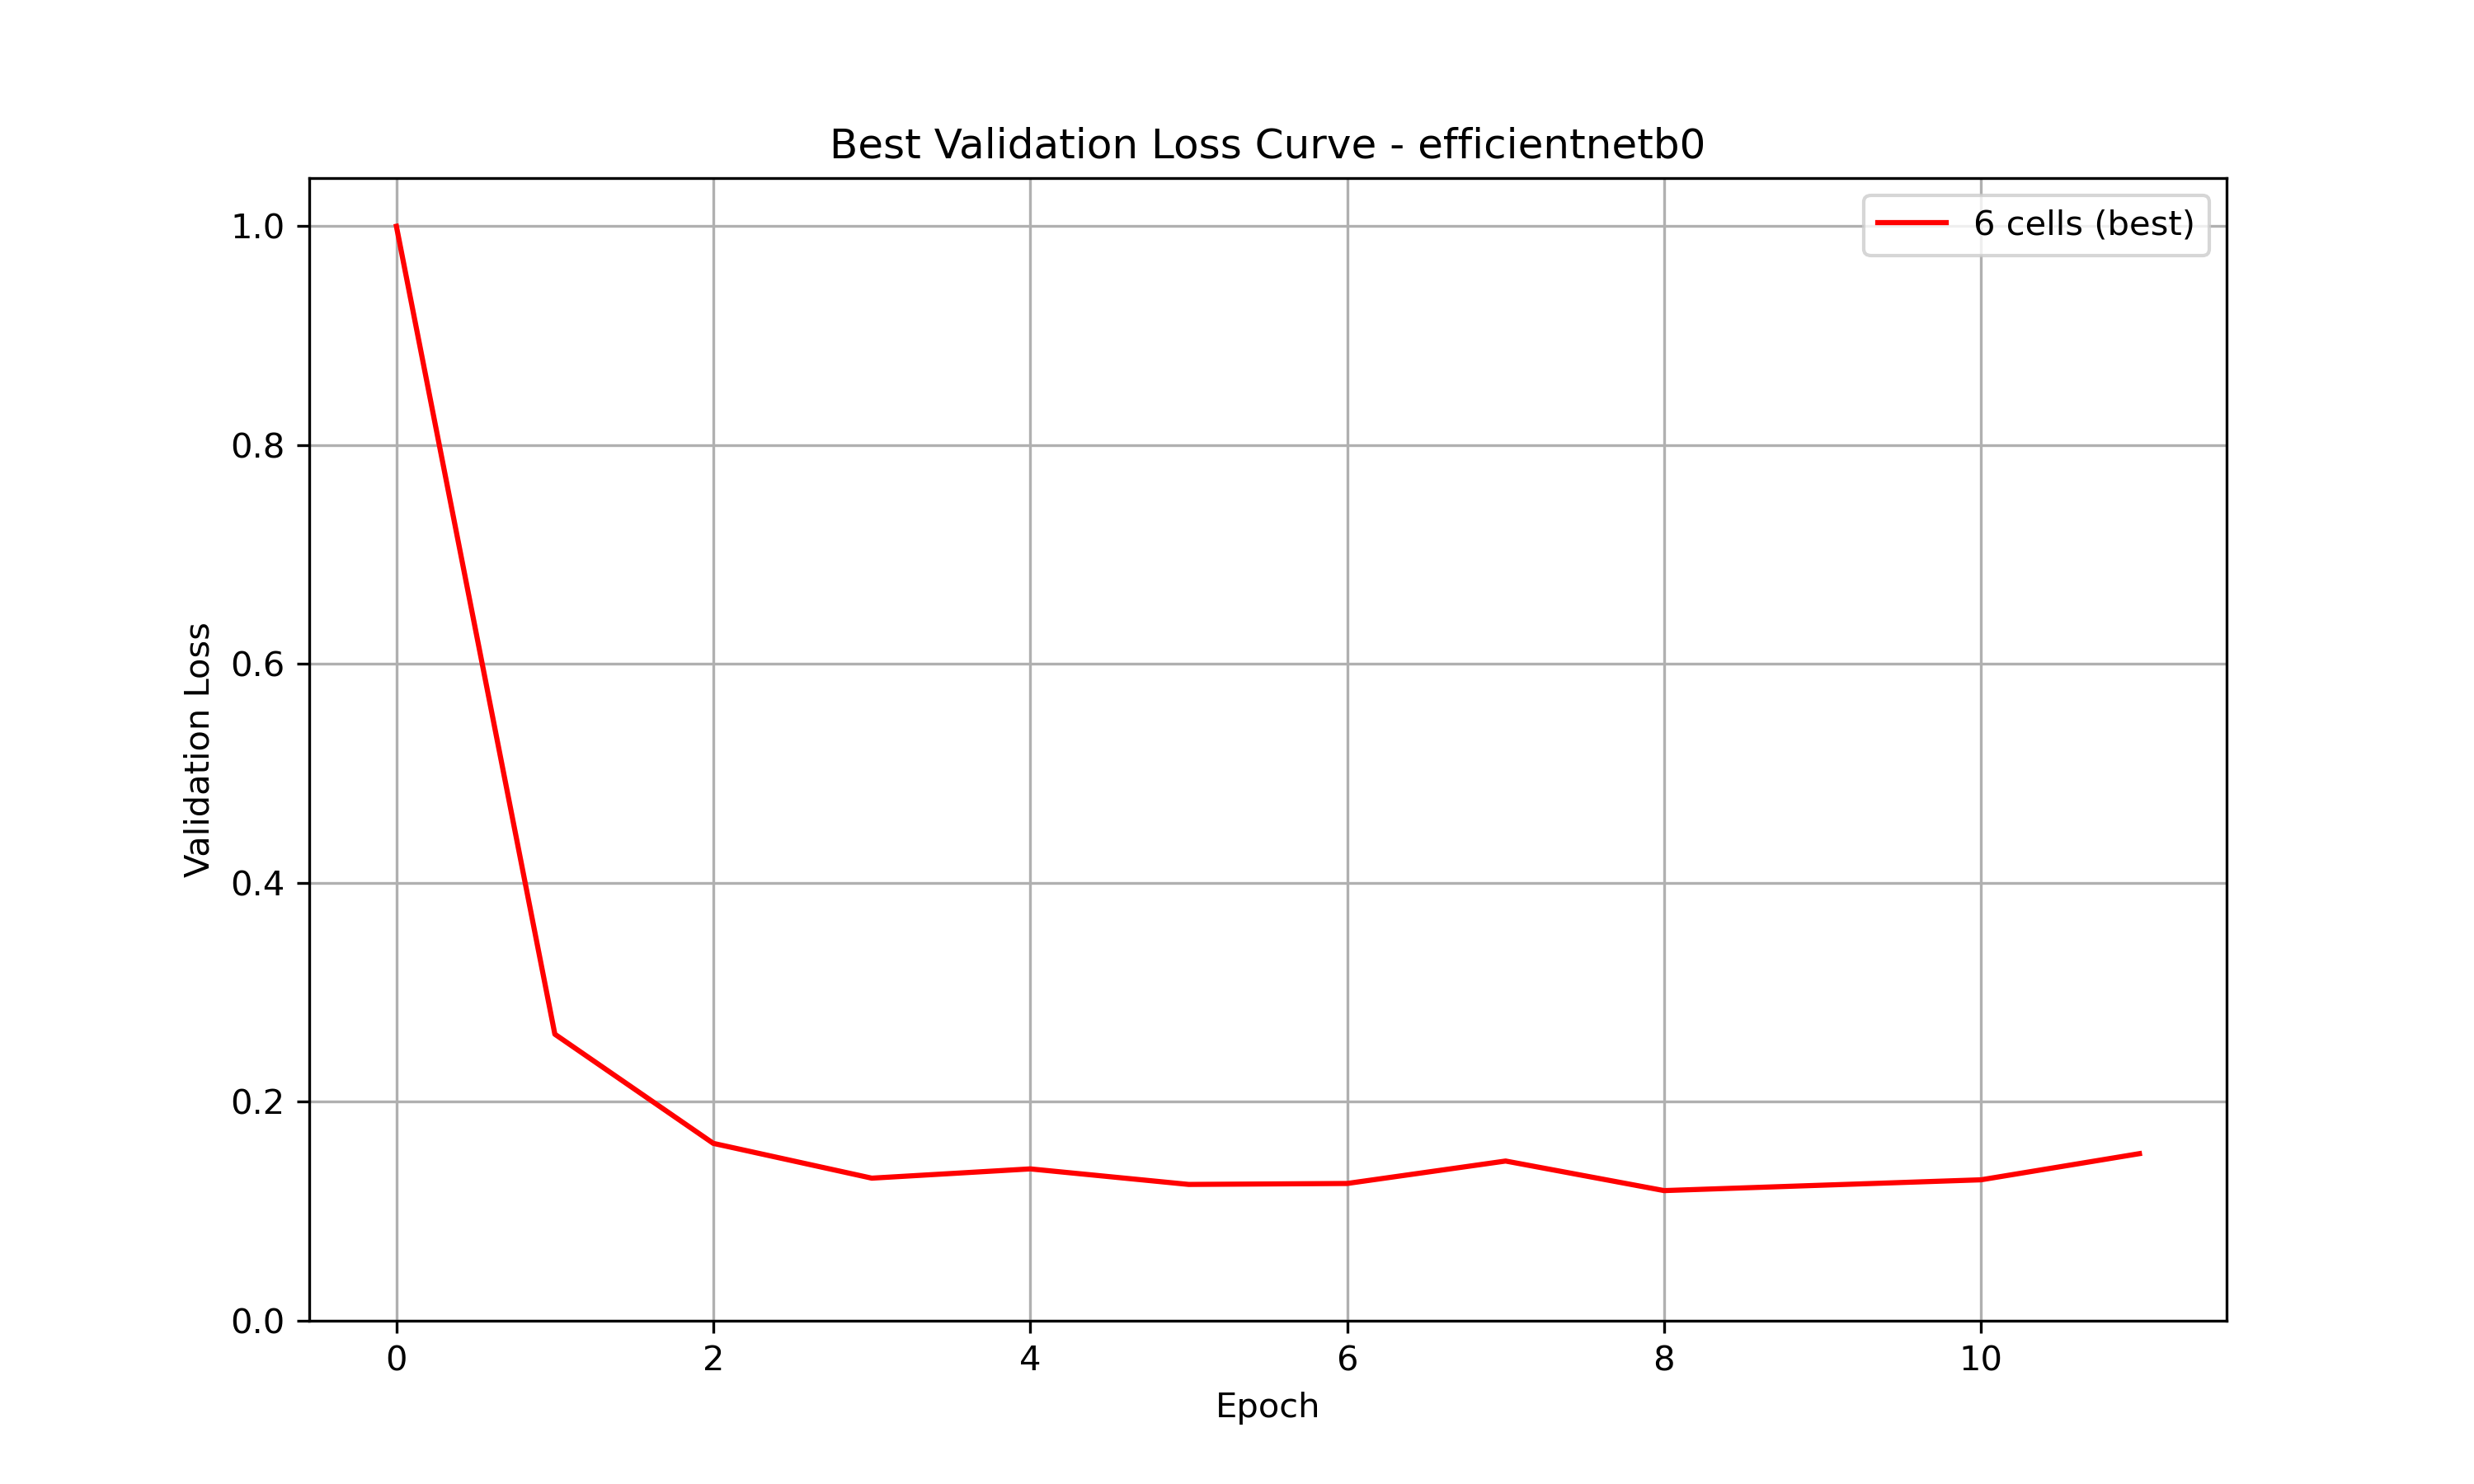
\includegraphics[width=0.8\textwidth]{../graphs/efficientnetb0_best_val_loss.png}
    \centering 
    \caption{Pérdida por época de EfficientNetB0 y 6 capas Bi-LSTM } 
    \label{EfficientNetB0Loss} 
\end{figure}


Los gráficos de las Figuras \ref{EfficientNetB0Accuracy} y 
\ref{EfficientNetB0Loss} muestran lo anteriormente mencionado acerca de 
que el dataset es bastante sencillo como para entrenar un modelo 
para clasificarlo. Durante la primera época, la pérdida baja a alrededor 
de 0.25 mientras que el accuracy logra llegar a 95\% en validación, 
lo cual indica que no está sobreajustandose a los datos de entrenamiento.\\ 

\textbf{\underline{Resultados obtenidos con EfficinetnetV2}}\\

De la misma manera, la Tabla  \ref{table:efficientnetV2Metrics} 
muestra una comparativa entre los resultados obtenidos para el 
\textit{pipeline} manteniendo los vectores de características 
obtenidas a través de EfficientNetV2 de los frames del 
\textit{dataset Hockey Fights}.

\begin{table}[h!]
\centering
\footnotesize
\caption{Métricas obtenidas por configuración de celdas para EfficientNetV2.}
\begin{tabular}{|l|l|l|l|l|l|l|}
\hline
\textbf{\begin{tabular}[c]{@{}l@{}}Celdas \\ Bi-LSTM\end{tabular}} & \textbf{\begin{tabular}[c]{@{}l@{}}Perdida \\ entrenamiento\end{tabular}} & \textbf{\begin{tabular}[c]{@{}l@{}}Accuracy \\ entrenamiento\end{tabular}} & \textbf{\begin{tabular}[c]{@{}l@{}}Perdida \\ validacion\end{tabular}} & \textbf{\begin{tabular}[c]{@{}l@{}}Accuracy \\ validacion\end{tabular}} & \textbf{\begin{tabular}[c]{@{}l@{}}Perdida \\ prueba\end{tabular}} & \textbf{\begin{tabular}[c]{@{}l@{}}Accuracy \\ prueba\end{tabular}} \\ \hline
\textbf{1}                                                         & 0.07                                                                      & 0.99                                                                       & 0.23                                                                   & 0.94                                                                    & 0.11                                                               & 0.97                                                                \\ \hline
\textbf{2}                                                         & 0.08                                                                      & 0.98                                                                       & 0.22                                                                   & 0.94                                                                    & 0.15                                                               & 0.96                                                                \\ \hline
\textbf{3}                                                         & 0.07                                                                      & 0.98                                                                       & 0.26                                                                   & 0.94                                                                    & 0.1                                                                & 0.96                                                                \\ \hline
\textbf{4}                                                         & 0.05                                                                      & 0.99                                                                       & 0.42                                                                   & 0.89                                                                    & 0.09                                                               & 0.98                                                                \\ \hline
\textbf{5}                                                         & \textbf{0.02}                                                             & \textbf{1.0}                                                               & 0.23                                                                   & 0.94                                                                    & \textbf{0.06}                                                      & \textbf{0.99}                                                       \\ \hline
\textbf{6}                                                         & 0.08                                                                      & 0.97                                                                       & 0.34                                                                   & 0.94                                                                    & 0.08                                                               & 0.98                                                                \\ \hline
\textbf{7}                                                         & 0.03                                                                      & 0.99                                                                       & 0.18                                                                   & 0.96                                                                    & 0.08                                                               & 0.98                                                                \\ \hline
\textbf{8}                                                         & 0.1                                                                       & 0.96                                                                       & 0.18                                                                   & 0.94                                                                    & 0.14                                                               & 0.95                                                                \\ \hline
\textbf{9}                                                         & 0.04                                                                      & 0.99                                                                       & \textbf{0.16}                                                          & \textbf{0.96}                                                           & 0.09                                                               & 0.97                                                                \\ \hline
\end{tabular}
\label{table:efficientnetV2Metrics}
\end{table}

En la Tabla \ref{table:efficientnetV2Metrics} se puede observar 
que la configuración que obtuvo el mejor desempeño general fue 
la de 5 celdas Bi-LSTM, alcanzando un \textit{accuracy} del 99\% 
en la prueba. En general, se puede ver que los resultados se mantienen 
consistentes entre configuraciones, con una leve caída en 
rendimiento en el extremo superior con 9 celdas, que mostró el peor 
resultado en prueba (97\% de \textit{accuracy}). Esto sugiere que 
aumentar el número de celdas o introducir un menor número puede 
introducir ruido o sobreajuste.\\

A continuación se presentan las gráficas de pérdida y 
\textit{accuracy} correspondientes a esta configuración óptima.

\begin{figure}[h!] 
    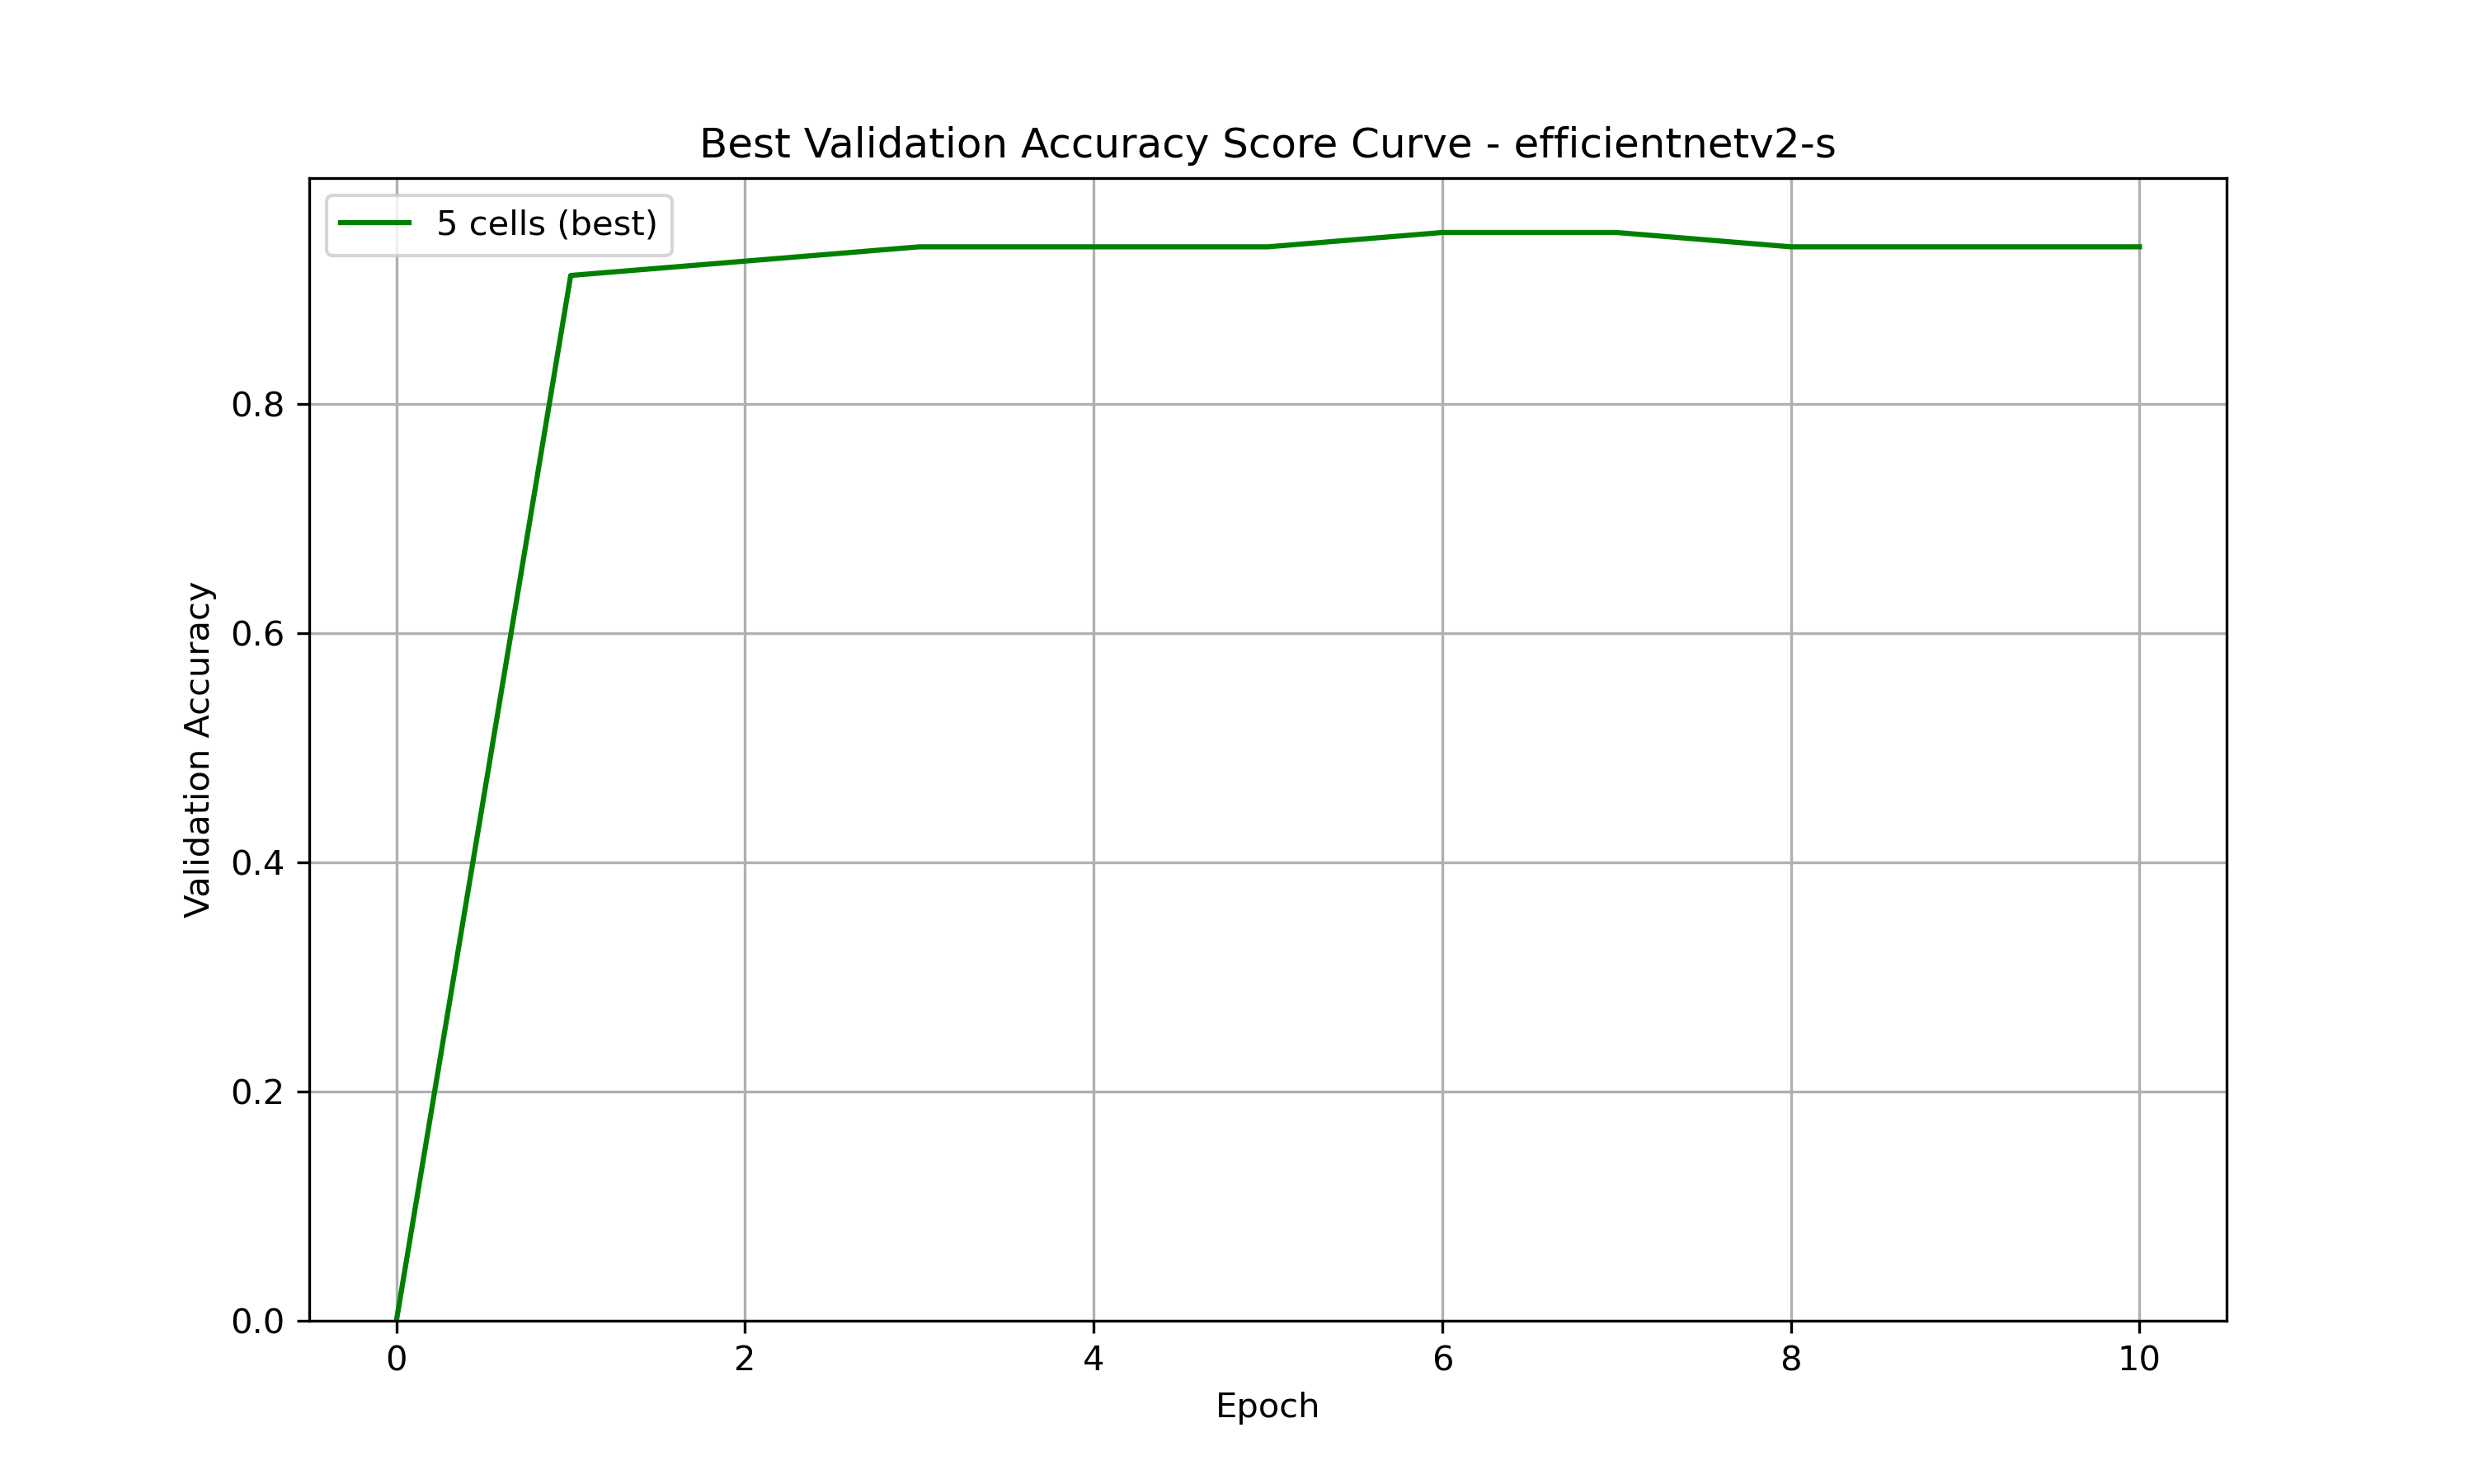
\includegraphics[width=0.8\textwidth]{../graphs/efficientnetv2-s_best_val_accuracy.png} 
    \centering 
    \caption{\textit{Accuracy} por época de EfficientNetV2 y 5 capas Bi-LSTM } 
    \label{EfficientNetV2Accuracy} 
\end{figure}

\begin{figure}[h!] 
    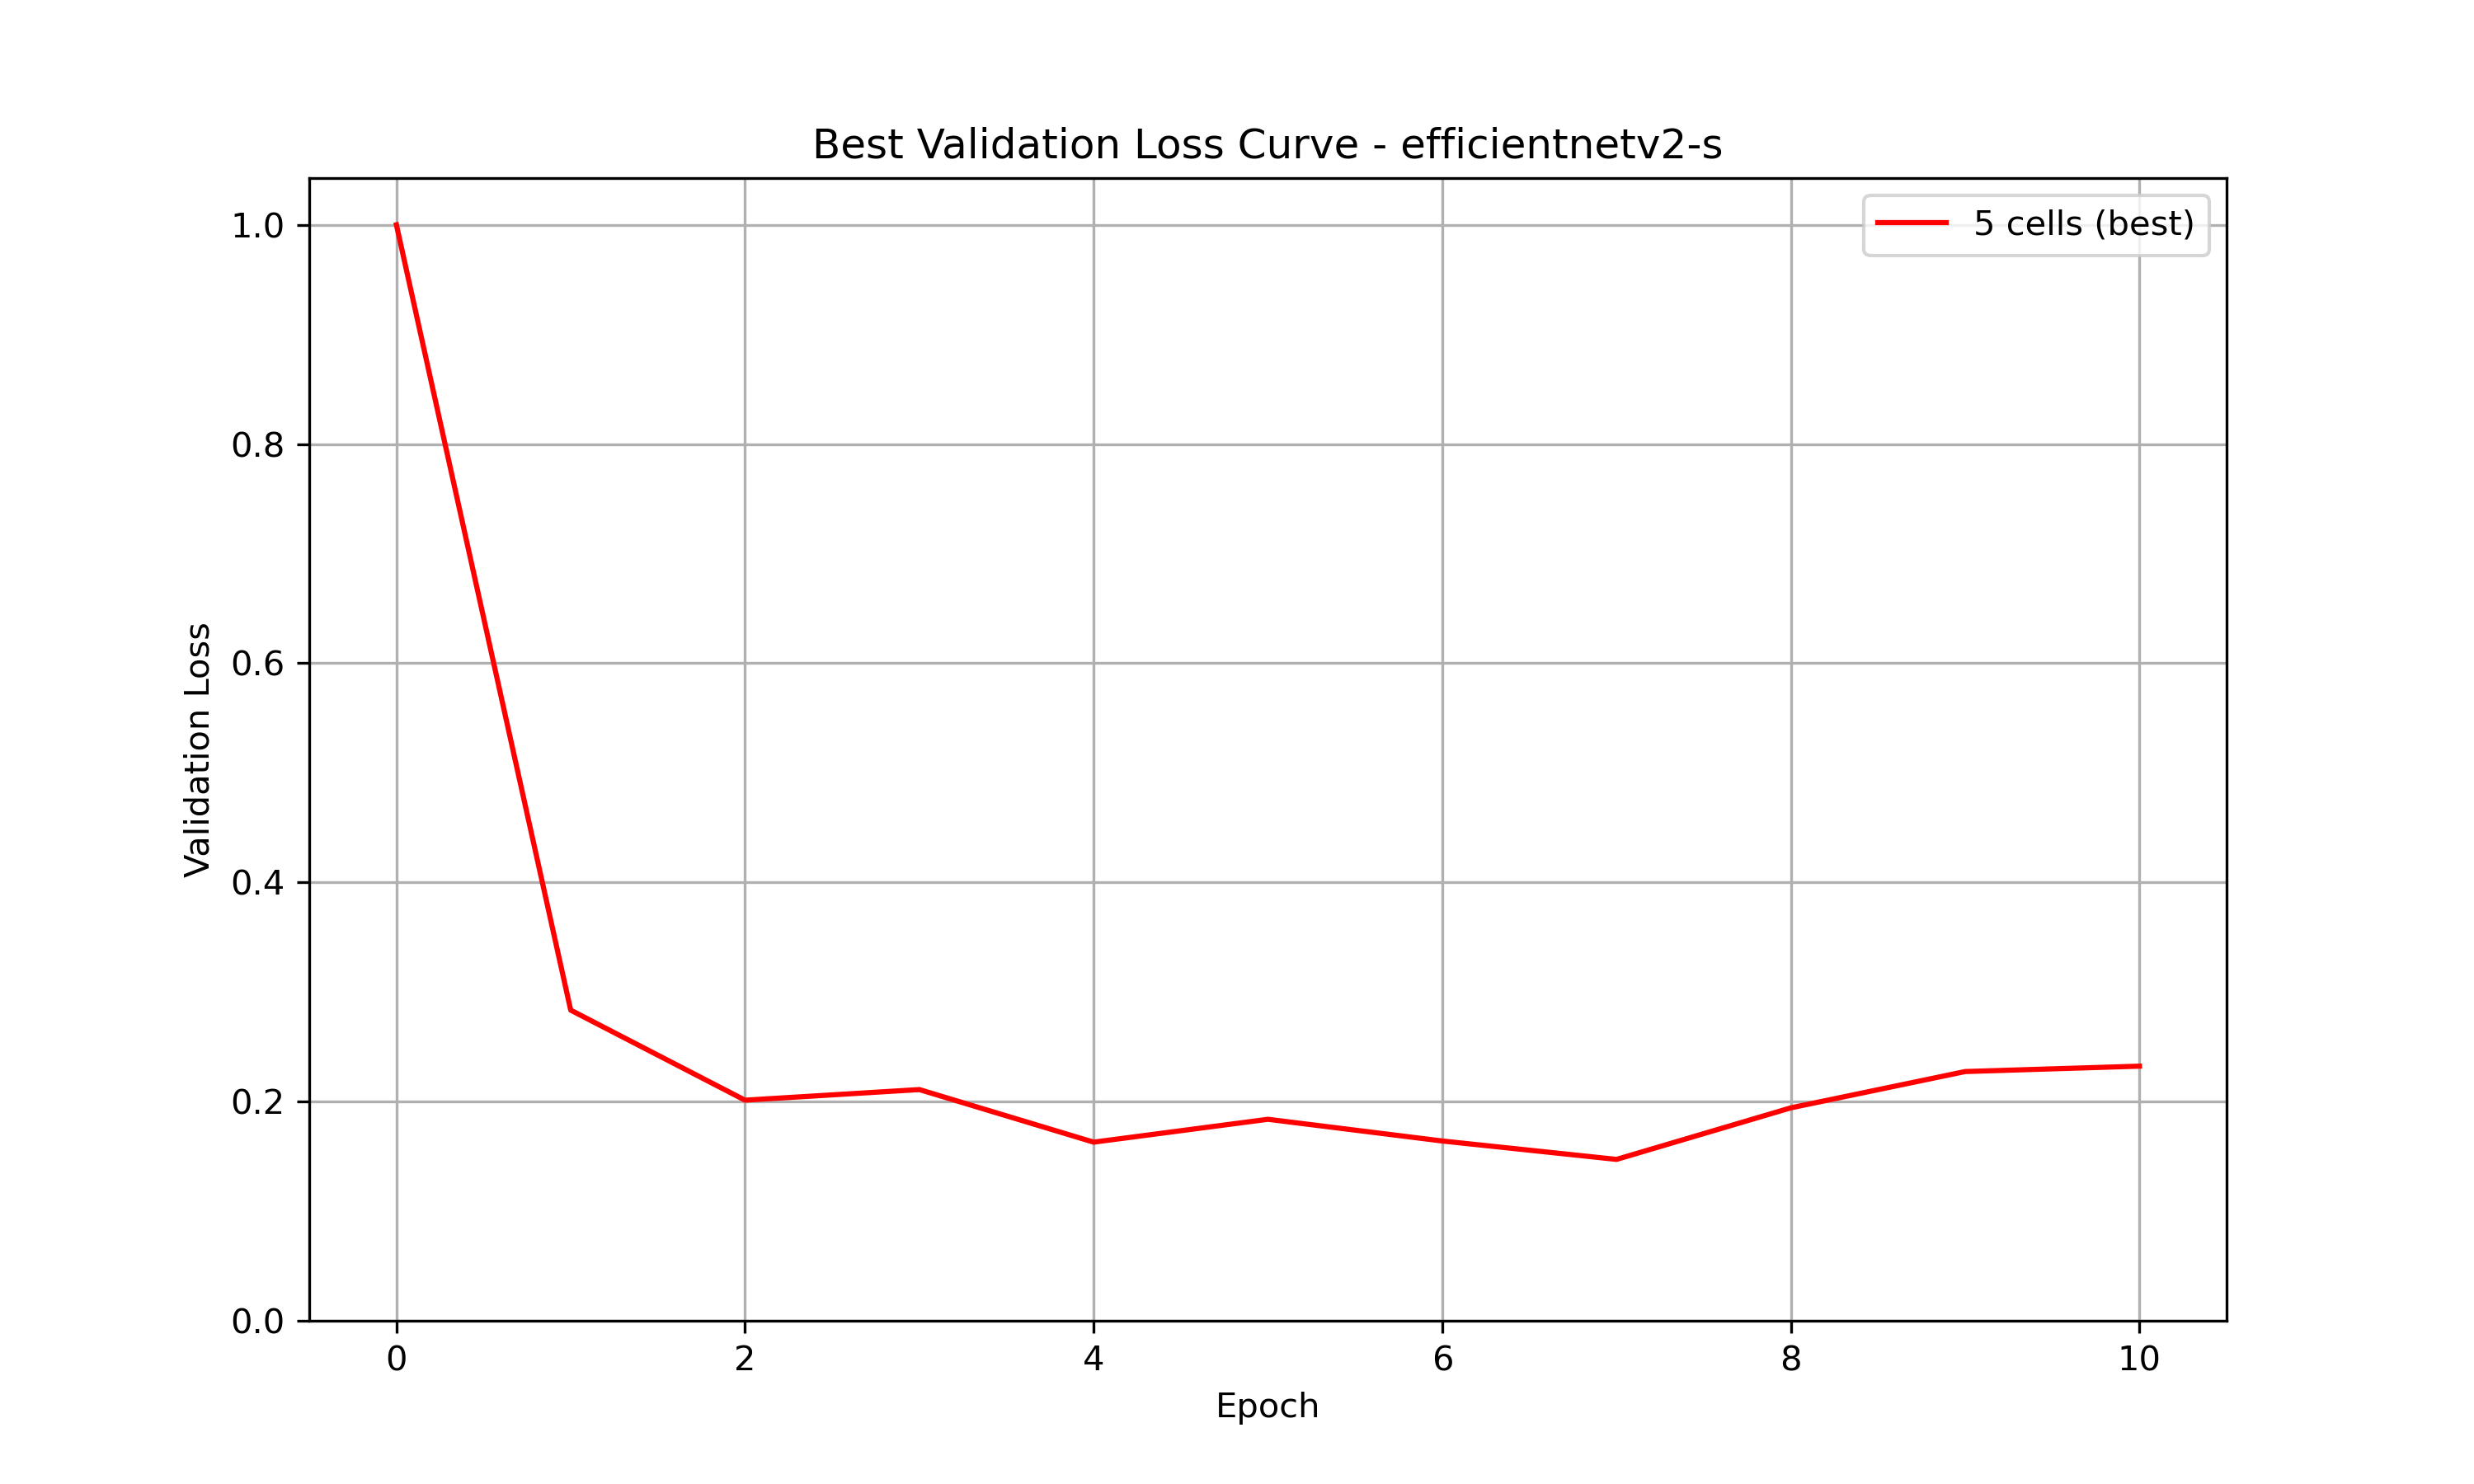
\includegraphics[width=0.8\textwidth]{../graphs/efficientnetv2-s_best_val_loss.png}
    \centering 
    \caption{Pérdida por época de EfficientNetV2 y 5 capas Bi-LSTM } 
    \label{EfficientNetV2Loss} 
\end{figure}


De la misma manera, Los gráficos de las Figuras \ref{EfficientNetV2Accuracy} y 
\ref{EfficientNetV2Loss} muestran el mismo patrón mencionado con los 
experimentos realizados con EfficientNetB0, en donde se obtiene un 
descenso de pérdida y aumento de \textit{accuracy} bastante rápido desde 
la primera época. Durante esta, la pérdida baja a alrededor 
de 0.35 mientras que el accuracy logra llegar a 90\% en validación, 
lo cual indica que no está sobreajustandose a los datos de entrenamiento.\\ 

\textbf{\underline{Resultados obtenidos con MobileNetV3}}\\

A continuación se muestra la Tabla \ref{table:MobileNetV3Metrics} 
la cual conteniendo los resultados obtenidos para el 
\textit{pipeline} manteniendo los vectores de características 
obtenidas a través de \textit{MobileNetV3} de los frames del 
\textit{dataset Hockey Fights}.

\begin{table}[h!]
\centering
\footnotesize
\caption{Métricas obtenidas por configuración de celdas para MobileNetV3.}
\begin{tabular}{|l|l|l|l|l|l|l|}
\hline
\textbf{\begin{tabular}[c]{@{}l@{}}Celdas \\ Bi-LSTM\end{tabular}} & \textbf{\begin{tabular}[c]{@{}l@{}}Perdida \\ entrenamiento\end{tabular}} & \textbf{\begin{tabular}[c]{@{}l@{}}Accuracy \\ entrenamiento\end{tabular}} & \textbf{\begin{tabular}[c]{@{}l@{}}Perdida \\ validacion\end{tabular}} & \textbf{\begin{tabular}[c]{@{}l@{}}Accuracy \\ validacion\end{tabular}} & \textbf{\begin{tabular}[c]{@{}l@{}}Perdida \\ prueba\end{tabular}} & \textbf{\begin{tabular}[c]{@{}l@{}}Accuracy \\ prueba\end{tabular}} \\ \hline
\textbf{1}                                                         & 0.18                                                                      & 0.94                                                                       & 0.24                                                                   & 0.93                                                                    & 0.18                                                               & 0.95                                                                \\ \hline
\textbf{2}                                                         & 0.04                                                                      & \textbf{0.99}                                                              & 0.2                                                                    & 0.94                                                                    & 0.08                                                               & 0.98                                                                \\ \hline
\textbf{3}                                                         & \textbf{0.02}                                                             & \textbf{0.99}                                                              & 0.24                                                                   & 0.95                                                                    & 0.07                                                               & 0.98                                                                \\ \hline
\textbf{4}                                                         & 0.06                                                                      & 0.98                                                                       & \textbf{0.15}                                                          & \textbf{0.96}                                                           & 0.1                                                                & 0.98                                                                \\ \hline
\textbf{5}                                                         & 0.05                                                                      & \textbf{0.99}                                                              & 0.18                                                                   & 0.95                                                                    & 0.1                                                                & 0.97                                                                \\ \hline
\textbf{6}                                                         & 0.07                                                                      & 0.98                                                                       & 0.18                                                                   & 0.94                                                                    & 0.11                                                               & 0.96                                                                \\ \hline
\textbf{7}                                                         & 0.03                                                                      & \textbf{0.99}                                                              & 0.19                                                                   & 0.94                                                                    & 0.08                                                               & 0.97                                                                \\ \hline
\textbf{8}                                                         & 0.06                                                                      & 0.98                                                                       & 0.23                                                                   & 0.94                                                                    & 0.17                                                               & 0.94                                                                \\ \hline
\textbf{9}                                                         & 0.06                                                                      & 0.98                                                                       & 0.19                                                                   & 0.95                                                                    & \textbf{0.05}                                                      & \textbf{0.99}                                                       \\ \hline
\end{tabular}
\label{table:MobileNetV3Metrics}
\end{table}

A comparación de los anteriores dos experimentos, no se logró ver 
ningún patrón característico con respecto al número de capas y la pérdida 
o el \textit{accuracy}. De la misma manera, no se obtuvo un modelo 
sobresaliente en cada una de las etapas de entrenamiento, validación y 
prueba. En ese sentido, se consideró como el mejor modelo al de 9 celdas 
Bi-LSTM debido a su \textit{accuracy} final en prueba, y a continuación 
se muestran las gráficas de pérdida y 
\textit{accuracy} correspondientes.\\

\begin{figure}[h!] 
    \includegraphics[width=0.8\textwidth]{../graphs/MobileNetV3large_best_val_accuracy.png} 
    \centering 
    \caption{\textit{Accuracy} por época de MobileNetV3 y 5 capas Bi-LSTM } 
    \label{MobileNetV3Accuracy} 
\end{figure}

\begin{figure}[h!] 
    \includegraphics[width=0.8\textwidth]{../graphs/MobileNetV3large_best_val_loss.png}
    \centering 
    \caption{Pérdida por época de MobileNetV3 y 5 capas Bi-LSTM } 
    \label{MobileNetV3Loss} 
\end{figure}

A comparación de las otras gráficas se logra ver un entrenamiento menos 
parejos, sobretodo si se ve la Figura \ref{MobileNetV3Loss} en donde 
llegado a la época 4, la gráfica se vuelve anómala en el entrenamiento. \\

\textbf{\underline{Resultados obtenidos con Resnet50}}\\

A continuación se muestra la Tabla  \ref{table:ResNet50} 
la cual conteniendo los resultados obtenidos para el 
\textit{pipeline} manteniendo los vectores de características 
obtenidas a través de \textit{Resnet50} de los frames del 
\textit{dataset Hockey Fights}.\\

\begin{table}[h!]
\centering
\footnotesize
\caption{Métricas obtenidas por configuración de celdas para ResNet50.}
\begin{tabular}{|l|l|l|l|l|l|l|}
\hline
\textbf{\begin{tabular}[c]{@{}l@{}}Celdas \\ Bi-LSTM\end{tabular}} & \textbf{\begin{tabular}[c]{@{}l@{}}Perdida \\ entrenamiento\end{tabular}} & \textbf{\begin{tabular}[c]{@{}l@{}}Accuracy \\ entrenamiento\end{tabular}} & \textbf{\begin{tabular}[c]{@{}l@{}}Perdida \\ validacion\end{tabular}} & \textbf{\begin{tabular}[c]{@{}l@{}}Accuracy \\ validacion\end{tabular}} & \textbf{\begin{tabular}[c]{@{}l@{}}Perdida \\ prueba\end{tabular}} & \textbf{\begin{tabular}[c]{@{}l@{}}Accuracy \\ prueba\end{tabular}} \\ \hline
\textbf{1}                                                         & 0.11                                                                      & 0.97                                                                       & \textbf{0.14}                                                          & \textbf{0.98}                                                           & 0.1                                                                & 0.97                                                                \\ \hline
\textbf{2}                                                         & 0.2                                                                       & 0.94                                                                       & 0.17                                                                   & 0.91                                                                    & 0.19                                                               & 0.94                                                                \\ \hline
\textbf{3}                                                         & 0.08                                                                      & 0.97                                                                       & 0.21                                                                   & 0.93                                                                    & 0.12                                                               & 0.96                                                                \\ \hline
\textbf{4}                                                         & 0.15                                                                      & 0.96                                                                       & 0.17                                                                   & 0.95                                                                    & 0.14                                                               & 0.96                                                                \\ \hline
\textbf{5}                                                         & 0.05                                                                      & 0.98                                                                       & \textbf{0.16}                                                          & \textbf{0.98}                                                           & 0.12                                                               & 0.97                                                                \\ \hline
\textbf{6}                                                         & 0.15                                                                      & 0.96                                                                       & 0.19                                                                   & 0.94                                                                    & 0.2                                                                & 0.95                                                                \\ \hline
\textbf{7}                                                         & \textbf{0.03}                                                             & \textbf{0.99}                                                              & \textbf{0.16}                                                          & 0.96                                                                    & \textbf{0.09}                                                      & \textbf{0.98}                                                       \\ \hline
\textbf{8}                                                         & 0.08                                                                      & 0.98                                                                       & 0.23                                                                   & 0.93                                                                    & 0.16                                                               & 0.94                                                                \\ \hline
\textbf{9}                                                         & 0.08                                                                      & 0.98                                                                       & \textbf{0.16}                                                          & 0.95                                                                    & 0.13                                                               & 0.96                                                                \\   \hline
\end{tabular}
\label{table:ResNet50}
\end{table}


En la Tabla \ref{table:ResNet50} se puede observar 
que la configuración que obtuvo el mejor desempeño casi general fue 
la de 7 celdas Bi-LSTM, alcanzando un \textit{accuracy} del 98\% 
en la prueba. En general, se puede ver que el rendimiento de los modelos 
decae conforme el número de celdas se aleja de 7 en todas las métricas, 
Esto sugiere también que aumentar el número de celdas o introducir 
un menor número puede introducir ruido o sobreajuste.

\begin{figure}[h!] 
    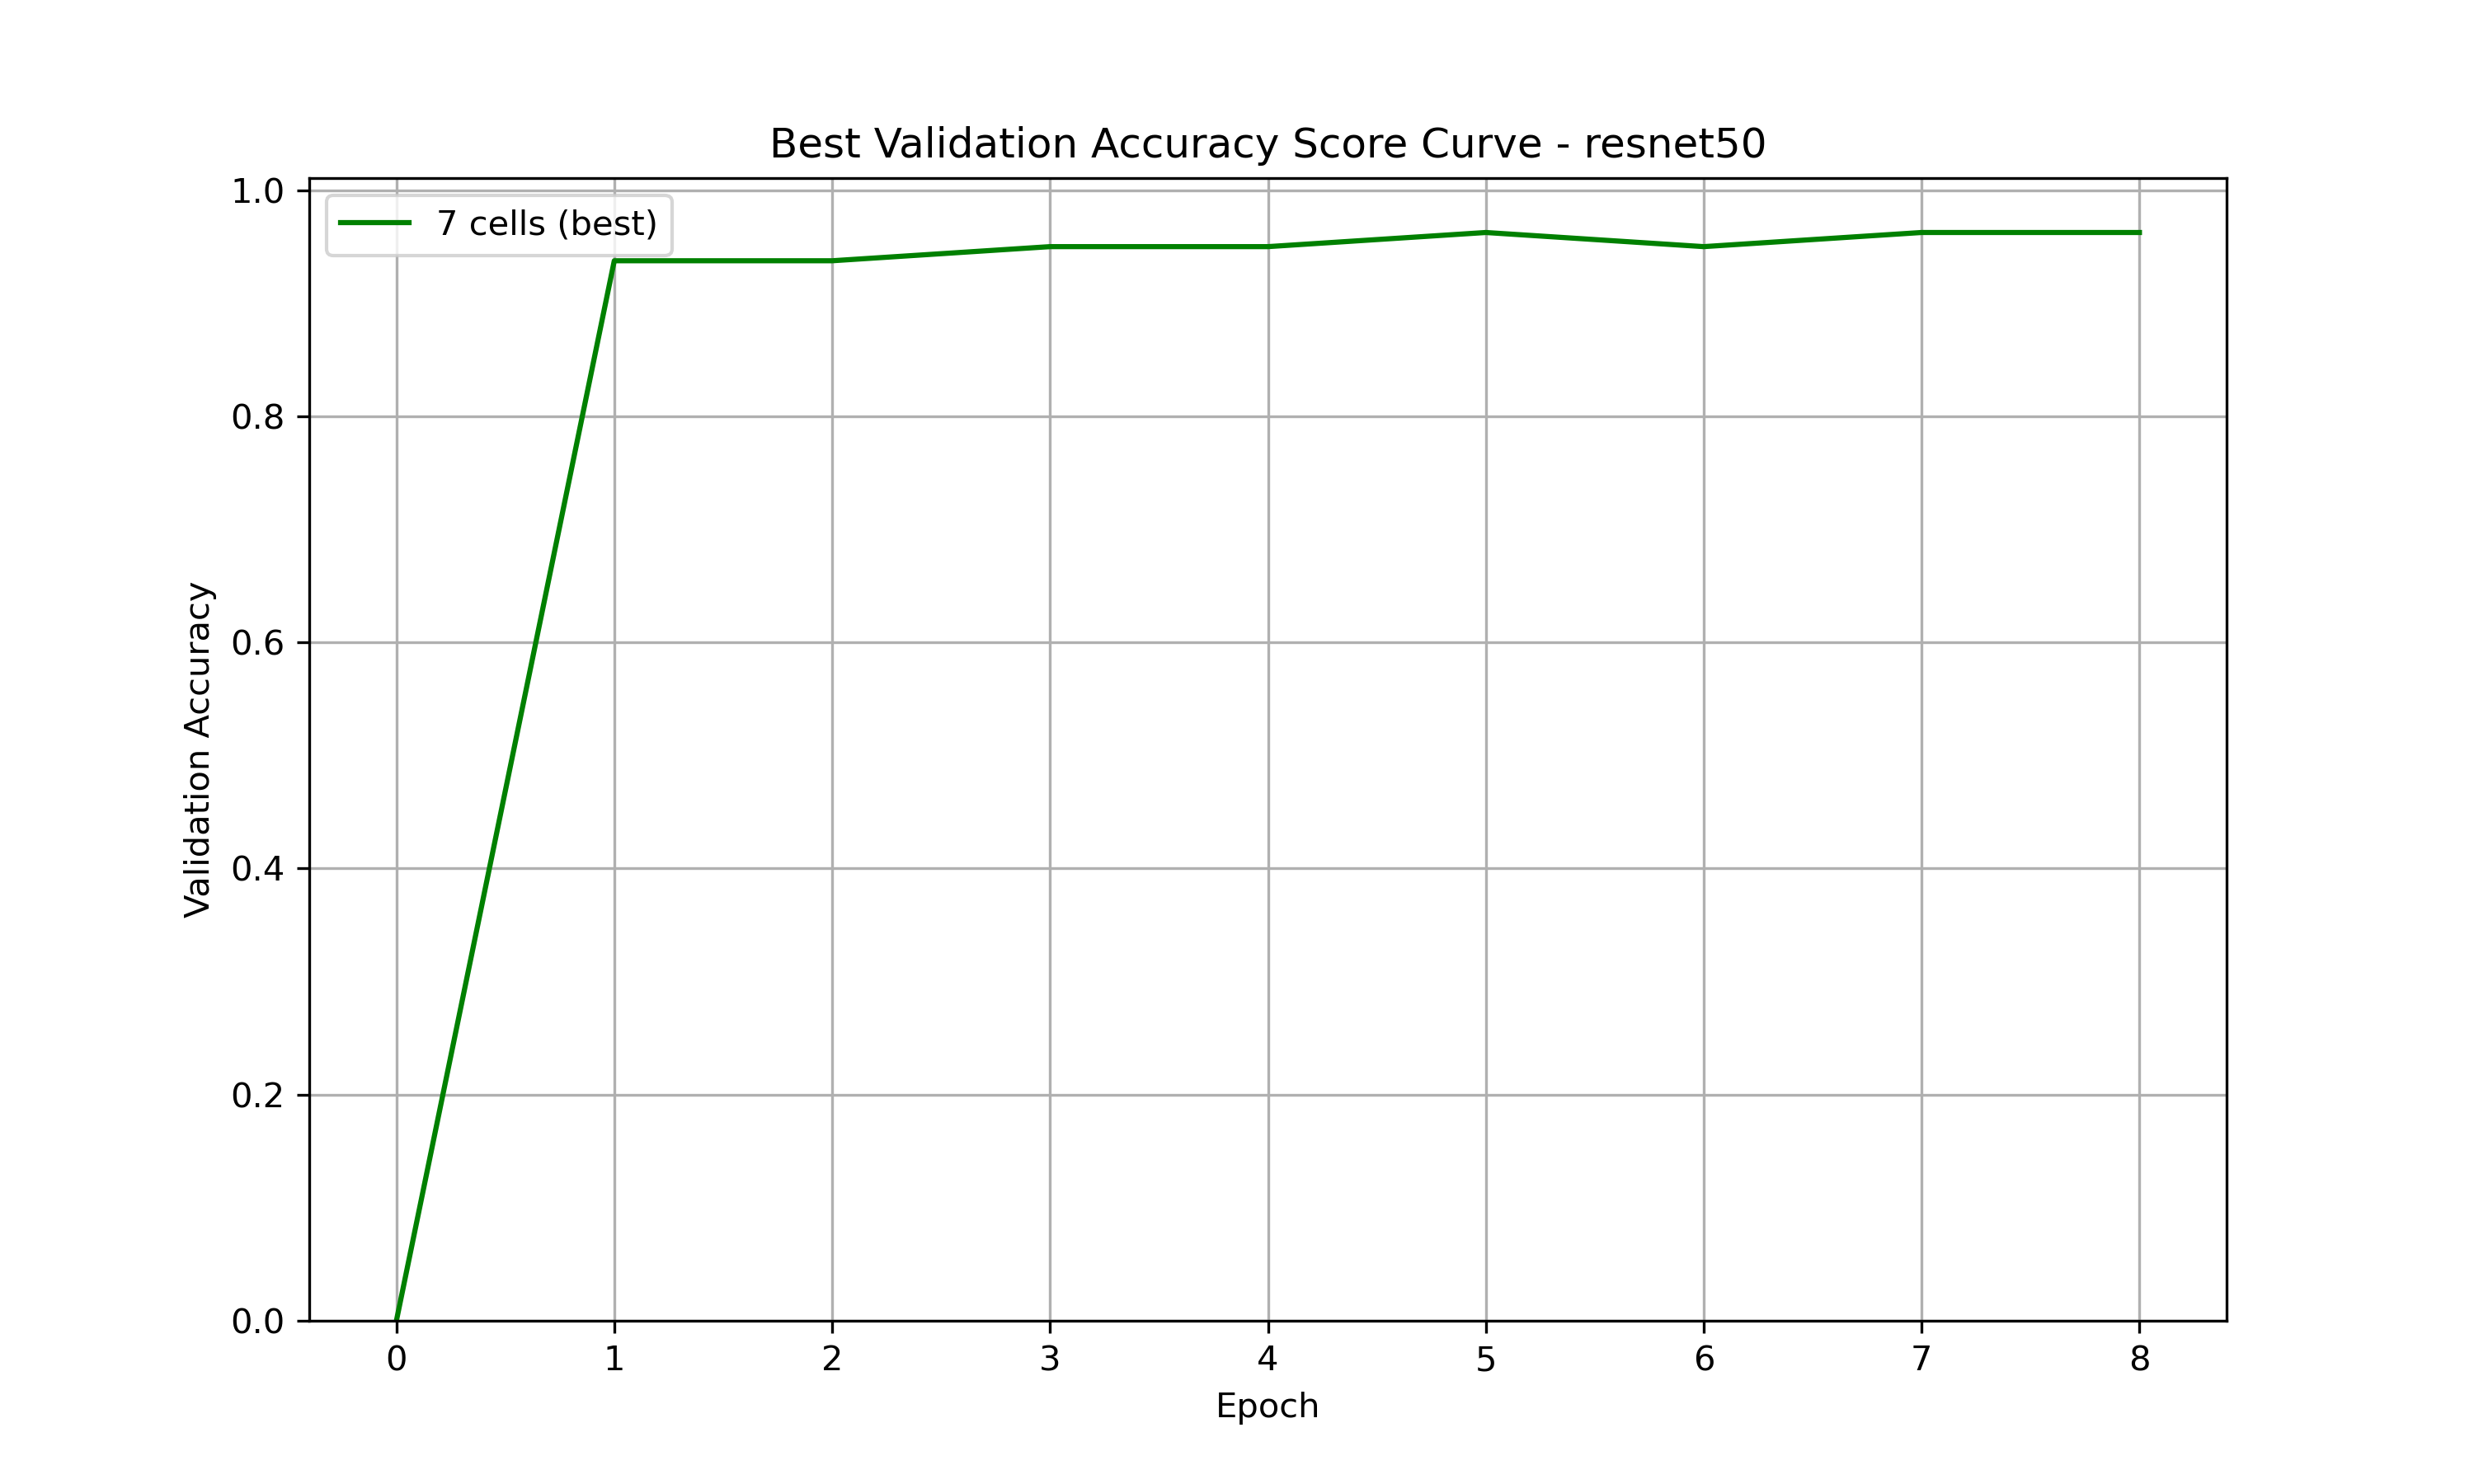
\includegraphics[width=0.8\textwidth]{../graphs/resnet50_best_val_accuracy.png} 
    \centering 
    \caption{\textit{Accuracy} por época de ResNet50 y 7 capas Bi-LSTM } 
    \label{ResNet50Accuracy} 
\end{figure}

\begin{figure}[h!] 
    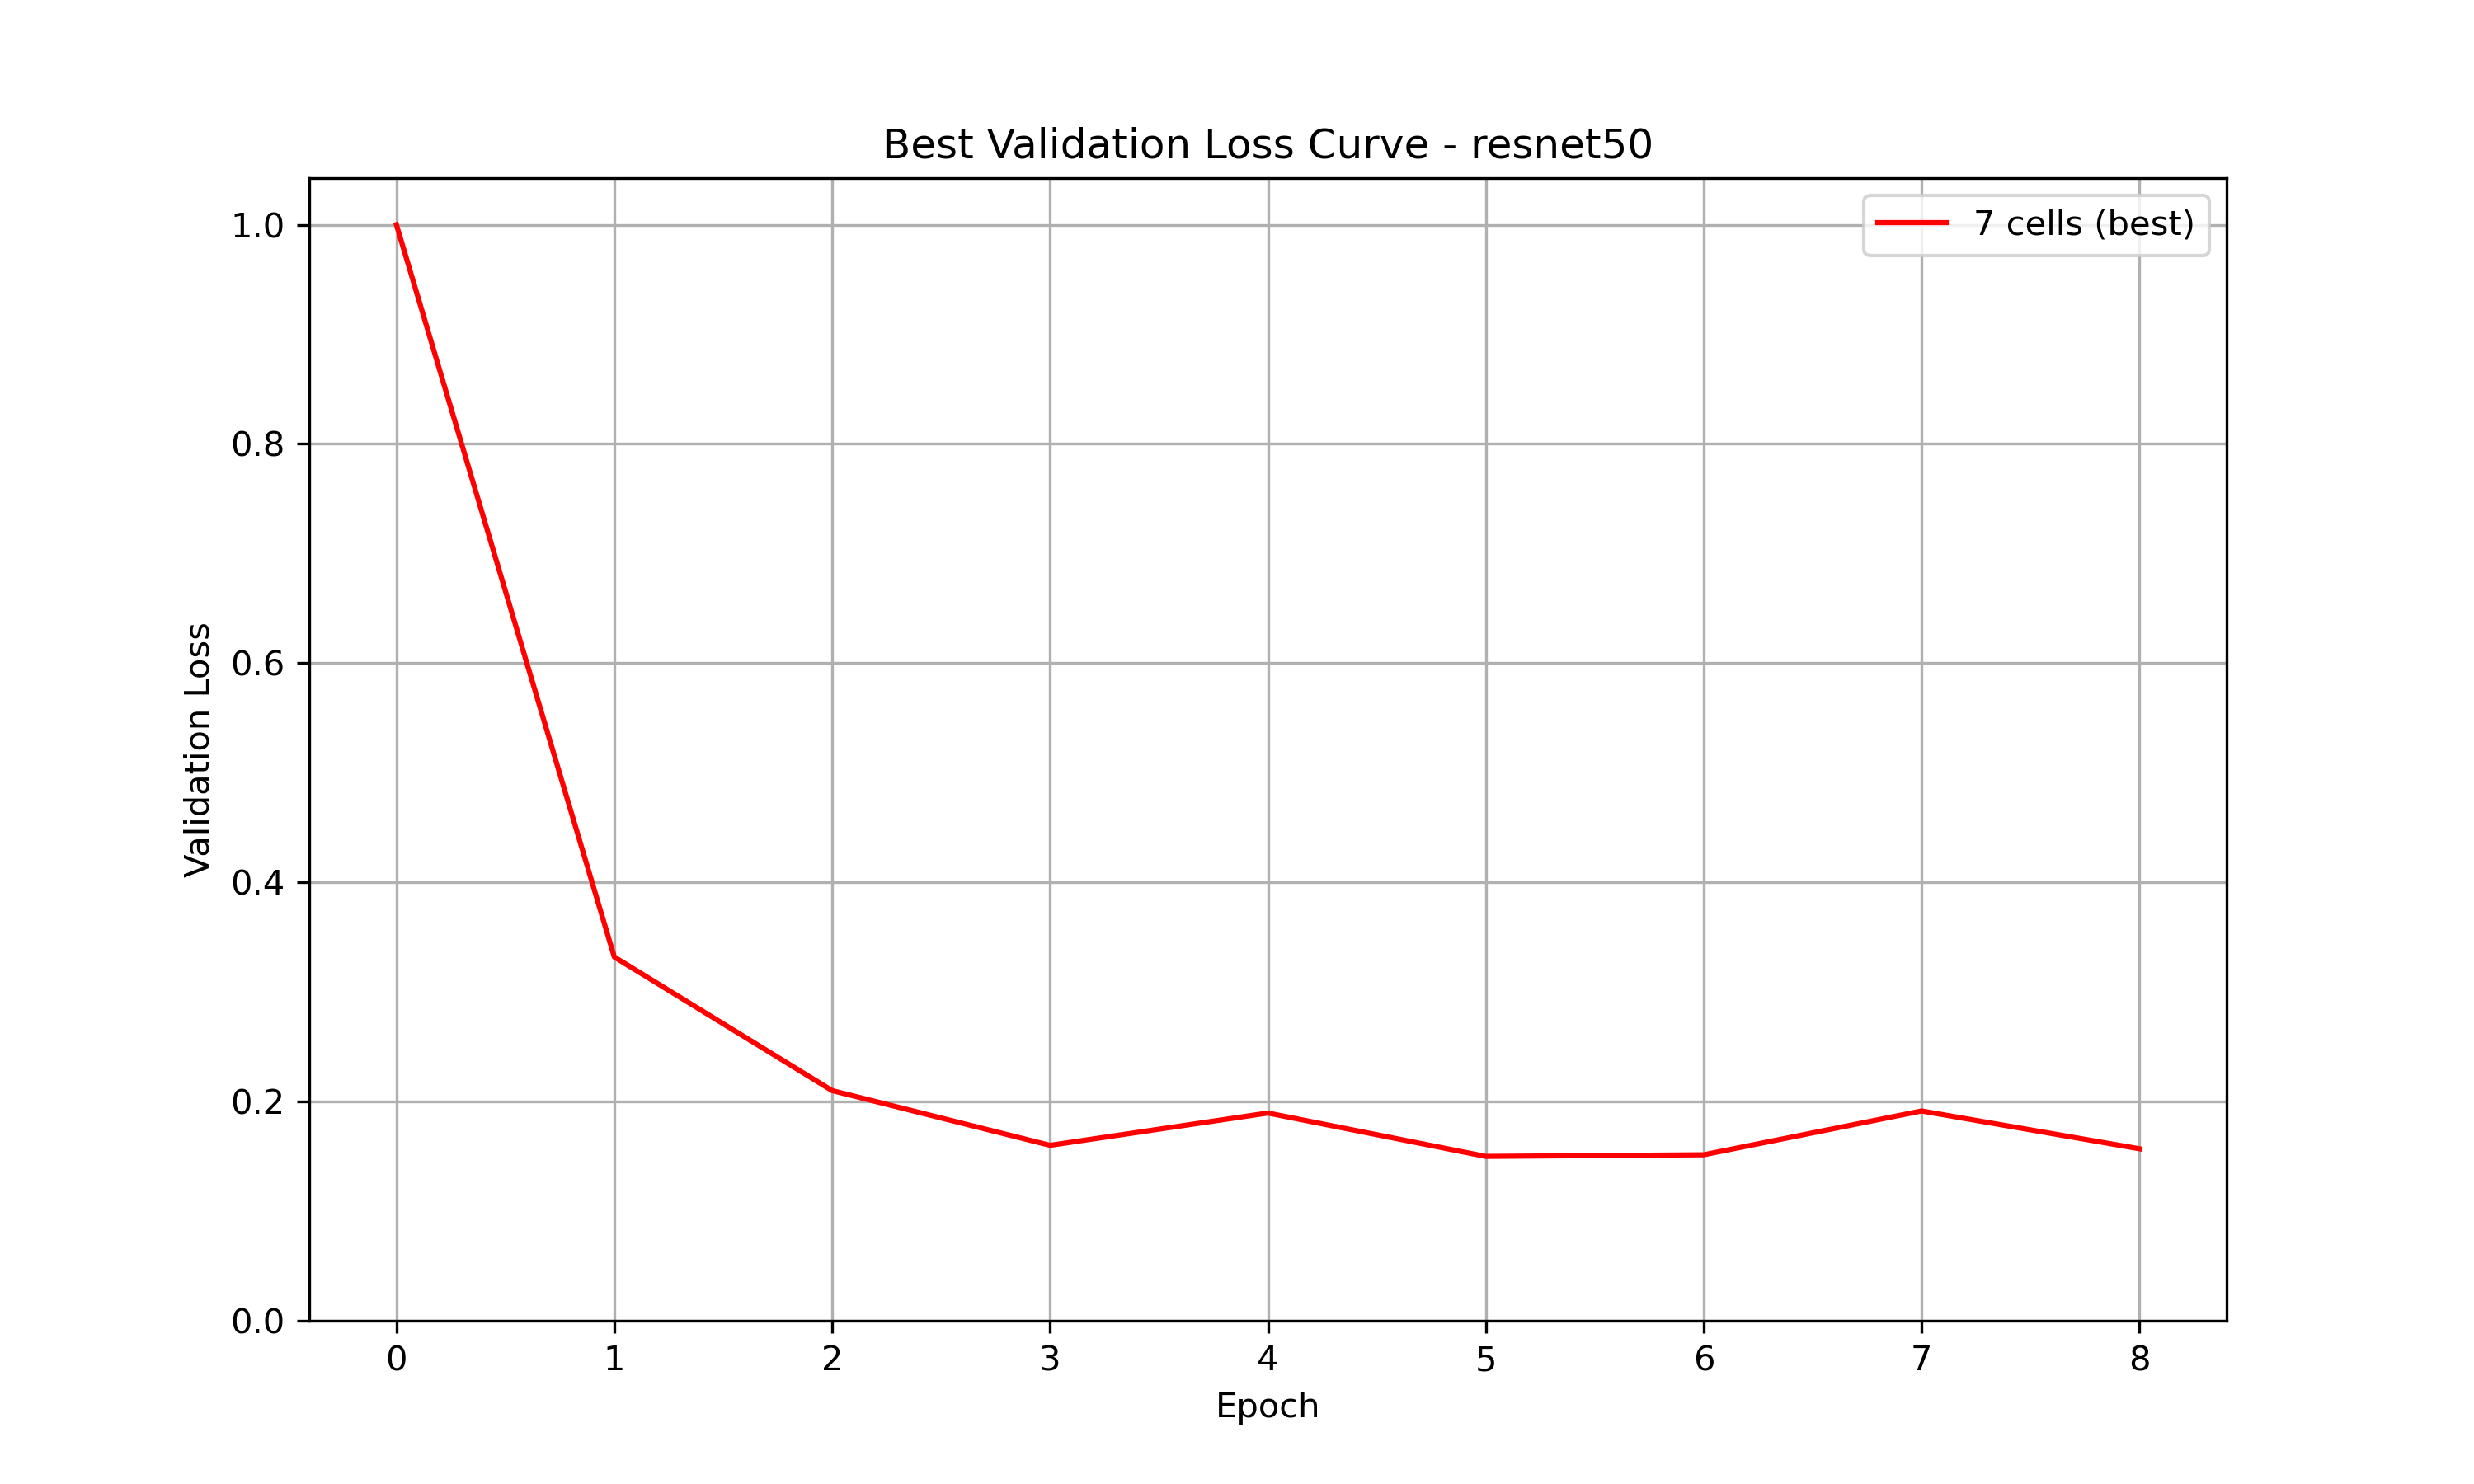
\includegraphics[width=0.8\textwidth]{../graphs/resnet50_best_val_loss.png}
    \centering 
    \caption{Pérdida por época de ResNet50 y 7 capas Bi-LSTM } 
    \label{ResNet50Loss} 
\end{figure}

Al igual que en la anterior experimentación, en la gráfica se logra ver 
un entrenamiento menos parejo, sobretodo si se ve la Figura 
\ref{ResNet50Loss} en donde llegado a la época 4, generando el mismo 
comportamiento anterior.\\

\subsection{Comparativa final}

A continuación se realizará una comparativa a modo de resumen  
de toda la experimentación realizada en el presente trabajo con 
los mejores resultados obtenidos. La Tabla \ref{table:comparacion} 
muestra todas las métricas utilizadas anteriormente para los mejores 
resultados de cada experimento.

\begin{table}[h!]
\centering
\caption{Tabla comparativa resumen final de la experimentación}
{\fontsize{6}{7}\selectfont
\begin{tabular}{|l|l|l|l|l|l|l|l|}
\hline
\multicolumn{1}{|c|}{\textbf{Modelo}} & \textbf{\begin{tabular}[c]{@{}l@{}}Pérdida \\ entrenamiento\end{tabular}} & \textbf{\begin{tabular}[c]{@{}l@{}}Capas \\ Bi-LSTM\end{tabular}} & \textbf{\begin{tabular}[c]{@{}l@{}}Accuracy \\ entrenamiento\end{tabular}} & \textbf{\begin{tabular}[c]{@{}l@{}}Pérdida \\ validación\end{tabular}} & \textbf{\begin{tabular}[c]{@{}l@{}}Accuracy \\ validación\end{tabular}} & \textbf{\begin{tabular}[c]{@{}l@{}}Pérdida \\ prueba\end{tabular}} & \textbf{\begin{tabular}[c]{@{}l@{}}Accuracy \\ prueba\end{tabular}} \\ \hline
\textbf{EfficientNetB0} & 6                    & \textbf{0.00}      & \textbf{1.00}             & \textbf{0.15}   & \textbf{0.98}     & \textbf{0.03}    & \textbf{0.99}     \\ \hline
\textbf{EfficientNetV2} & \textbf{5}           & 0.02               & \textbf{1.00}             & 0.23            & 0.94              & 0.06             & \textbf{0.99}   \\ \hline
\textbf{MobileNetV3}    & 9                    & 0.06               & 0.98                      & 0.19            & 0.95              & 0.05             & \textbf{0.99}   \\ \hline
\textbf{ResNet50}       & 7                    & 0.03               & 0.99                      & 0.16            & 0.96              & 0.09             & 0.98     \\ \hline
\end{tabular}
}
\label{table:comparacion}
\end{table}

Con los resultados finales se puede corroborar que todas las 
combinaciones entre CNN y Bi-LSTM lograron valores similares para 
todas las métricas de testeo al tener un \textit{accuracy} alto y similar 
(98-99\%). Aún así, es importante resaltar que en todas las métricas a lo 
largo del proceso de entrenamiento, validación y prueba, EfficientNetB0 
fue quien obtuvo los mejores resultados en comparación al resto 
(incluyendo el necesitar la menor cantidad de capas Bi-LSTM). En ese 
sentido, y con el fin de optimizar el \textit{pipeline} final de 
manera general, sería recomendable utilizar EfficientNetB0 como extractor 
de características. \\

Por otra parte, y basado en los resultados de todas 
las tablas comparativas anteriormente ilustradas, es recomendable tratar 
de encontrar la configuración con el número de celdas correcto, para 
optimizar el \textit{pipeline} final. Utilizando los patrones 
encontrados, se puede ver que las métricas van a ir mejorando conforme 
más capas se aumente, hasta cierto límite, siendo ese el número ideal 
de capas Bi-LSTM que se debe utilizar.

\chapter{Conclusiones y Trabajo Futuro}

En la Ecuación \eqref{eq:eq1secCTF}


\begin{equation}\label{eq:eq1secCTF}
M=\begin{pmatrix}
	m_{11}&m_{12}\\
	m_{21}&m_{22}
\end{pmatrix}
\end{equation}

En la siguiente Tabla \ref{tab:tab1secCTF}

\begin{table}[h]
\centering
\begin{tabular}{|c|c|}
	\hline
	1 & 2 \\
	\hline
	22 & 11 \\
	\hline
\end{tabular}
\caption{Tabla 1}
\label{tab:tab1secCTF}
\end{table}

En la siguiente Figura \ref{fig:fig1secCTF}

\begin{figure}[h]

\includegraphics[width= 0.8\textwidth]{logo_unir}
\caption{Logo Unir}
\label{fig:fig1secCTF}
\end{figure}

\cite{PIMENTEL2016744} \cite{da_S_Bessa_2023}


%\begin{thebibliography}{a}
%\bibitem{etiqueta} \textsc{Autores},
%\textit{nombre referencia.}
%Información addicional
%\end{thebibliography}
\newpage
\bibliography{bibliografia}

\appendix
\chapter{Apendices}

\end{document}





















